\documentclass[
	a4paper,
	english,
	twoside,
	openright,               
	11pt                            
	]{report}

\usepackage{textcomp}
\usepackage{listings}
\usepackage{pgfplots}

\usepackage[T1,OT1]{fontenc}
\usepackage[utf8]{inputenc}
\usepackage{subcaption}
\captionsetup{compatibility=false}
\usepackage{float}
\usepackage{chngcntr}
\usepackage{placeins}
\usepackage[ngerman,american]{babel}
\usepackage[toc,page]{appendix}
\usepackage{amssymb}
\usepackage{graphicx}
\usepackage{blindtext}
\usepackage{enumitem}
\usepackage{amsmath}
\usepackage[justification=centering]{caption}
\usepackage{glossaries}
\graphicspath{ {./img/} }
\PassOptionsToPackage{hyphens}{url}\usepackage{hyperref}
\setcounter{tocdepth}{3}
\pgfplotsset{compat=newest}

\begin{document}
%%%%%%%%%%%%%%%%%%%%%%%%%%%%%%%%%%%%%%%%%%%%%%%%%%%%%%%%%%%%%%%%%%%%%%
%%  Titelseite fuer eine Diplomarbeit/Dissertation an der Uni Wien  %%
%%                     zur Benutzung mit LaTeX                      %%
%%%%%%%%%%%%%%%%%%%%%%%%%%%%%%%%%%%%%%%%%%%%%%%%%%%%%%%%%%%%%%%%%%%%%%

%%  Erstellt anhand der Vorlagendefinition von
%%  http://www.univie.ac.at/Psychologie/cgi-bin/dbman/uploads/download/
%%      51_infoblatt__titelblatt_wissenschaftliche_arbeit.pdf
%%
%% Einzubinden in der eigenen document-Umgebung mittels \input{thesistitle}
%%
%% Ueberschriften wie "Titel der Diplomarbeit" oder "Verfasserin" (etc.)
%% muessen genau so stehen bleiben. Nur der Titel der Arbeit oder die Namen
%% sind entsprechend beliebig.

% Stephan Paukner, 14.08.2007
% Obige Vorlagendefinition schlaegt Arial oder eine vergleichbare serifenlose
% Schriftart vor. Der serifenlose Font von LaTeX, CMSS, hat leider keine
% fette (bold) Variante. Arial ist allerdings ein kommerzieller Font und unter
% LaTeX standardmaessig nicht verfuegbar. Am naehesten kommt dem der Font
% Helvetica, einzubinden via \usepackage[scaled=0.90]{helvet} in der Praeambel.

\begin{titlepage}
\vspace*{-2cm}  % bei Verwendung von vmargin.sty
\begin{flushright}
	
\includegraphics[width=.5\textwidth]{titlepage/RZ_Logo_Uni_sw_01.jpg}
\end{flushright}
\vspace{1cm}

\begin{center}  % Diplomarbeit ODER Magisterarbeit ODER Dissertation
    \huge{\textbf{\textsf{\MakeUppercase{
        MASTERARBEIT / MASTER'S THESIS
    }}}}
    \vspace{2cm}

    \large{\textsf{  % Diplomarbeit ODER Magisterarbeit ODER Dissertation
                     % (Dies ist erst die Ueberschrift!)
        Titel der Masterarbeit / Title of the Master's Thesis
    }}
    \vspace{.1cm}

    \LARGE{\textsf{  % Hier kommt der eigentliche Titel, bei Bedarf mit \\
                     % ACHTUNG: Deutsche Anfuehrungszeichen: ,,Titel``
                     %          English quotes:              ``title''
        % >>>>> BEGINN TITEL >>>>>
        {\glqq}Tool for Visual Cluster Analysis and Consensus Clustering\grqq
        %``The Creation of a Title Page''
        % <<<<< ENDE TITEL <<<<<
    }}
    \vspace{2cm}

    \large{\textsf{  % Verfasserin ODER Verfasser (Ueberschrift)
        verfasst von / submitted by
    }}

    \Large{\textsf{  % Vorname Nachname
        % >>>>> BEGINN VORNAME NACHNAME >>>>>
        Christian Permann, BSc
        % <<<<< ENDE VORNAME NACHNAME <<<<<
    }}
    \vspace{2cm}

    \large{\textsf{
        angestrebter akademischer Grad / in partial fulfilment of the requirements for the degree  % (Ueberschrift)
    }}

    \Large{\textsf{  % Magistra ODER Magister ODER Doktorin ODER Doktor
                     % ACHTUNG: Kuerzel "Mag.a" oder "Dr.in" nicht zulaessig
				Master of Science (MSc)
    }}
\end{center}
\vspace{2cm}

\noindent\textsf{Wien, 2020 / Vienna, 2020}  % <<<<< ORT, MONAT UND JAHR EINTRAGEN
\vfill

\noindent\begin{tabular}{@{}p{8cm}p{8cm}}
\textsf{Studienkennzahl lt. Studienblatt / }
&
\textsf{UA 066 921} % <<<<< STUDIENKENNZAHL LT. CURRICULUM EINTRAGEN
\\
\textsf{degree programme code as it appears on}
&
\\
\textsf{the student record sheet}
&
\\
\end{tabular}

\vspace{0.2cm}
    % BEI DISSERTATIONEN:
%\textsf{Dissertationsgebiet lt. Studienblatt:}
    % ANSONSTEN:
\noindent\begin{tabular}{@{}p{8cm}p{8cm}}
\textsf{Studienrichtung lt.\ Studienblatt:/}
&
\textsf{Masterstudium Informatik}  % <<<<< DISSGEBIET/STUDIENRICHTUNG EINTRAGEN
\\
\textsf{degree programme as it appears on}
&
\\
\textsf{the student record sheet}
&
\\
\end{tabular}

\vspace{0.2cm}

\noindent\begin{tabular}{@{}p{8cm}p{8cm}}
% Betreuerin ODER Betreuer:
\textsf{Betreut von / Supervisor:}
&
\textsf{Univ.-Prof. Dipl.-Inform.Univ. Dr. Claudia Plant}  % <<<<< NAME EINTRAGEN
\\
%&
%\textsf{2. Betreuer mit Titel}  % <<<<< NAME EINTRAGEN
%\textsf{degree(s) first name family name}
\end{tabular}

\end{titlepage}


% \newpage
%
% \thispagestyle{empty}
% \text{ }
% \vspace{13.5cm}
%
%
% Martin Perdacher\\
% Teybergasse 4/5\\
% 1140 Wien\\
%
% Hiermit versichere ich, dass ich die von mir vorgelegte Arbeit selbstständig verfasst habe, dass ich die verwendeten Quellen, Internet-Quellen und Hilfsmittel vollständig angegeben habe und dass ich die Stellen der Arbeit -- einschließlich Tabellen, Karten und Abbildungen~--, die anderen Werken oder dem Internet im Wortlaut oder dem Sinn nach entnommen sind, auf jeden Fall unter Angabe der Quelle als Entlehnung kenntlich gemacht habe.\\

% Wien, den 1. Dezember 2020\\
% \medskip
% \medskip
%
% (Unterschrift)\\
% \underline{~~~~~~~~~~~~~~~~~~~~~~~~~~~~~~~~~~~~~~~~}\\
% Martin Perdacher\\

%\newpage



\chapter*{Danksagungen} % (fold)
\label{cha:acknowledgements}
\noindent

Ich möchte meiner Betreuerin Univ.-Prof. Dipl.-Inform.Univ. Dr. Claudia Plant für Ihre Unterstützung bei dieser Arbeit danken. Unsere offenen und konstruktiven Gespräche haben mir sehr geholfen diese Arbeit zielstrebig und motiviert zu vollenden. Ebenso möchte ich Univ.-Prof. Torsten Möller, PhD meinen dank aussprechen. Die gemeinsamen Überlegungen zu dieser Arbeit haben sicherlich zu einem besseren Ergebnis geführt.

Ebenso ist es mir wichtig meinen Eltern, Eva Maria Pichler und Otto Permann, zu danken. Sie haben mich durch mein ganzes Leben unterstützt und es mir erst möglich gemacht beruflich als auch persönlich so weit zu kommen.

Große Unterstützung habe ich auch durch meine Freundin Rebecca Käfer erhalten, sie war immer für mich da, insbesondere wenn mir die universitäre Arbeit zu viel wurde. Hierfür bin ich besonders dankbar.

Auch meine Freunde und Studienkollegen waren maßgeblich für meinen Erfolg und mein Leben im allgemeinen. Der positive Umgang an unserer Fakultät, das leichte Anfreunden und die nahezu selbstverständliche gegenseitige Hilfe sind Aspekte von denen die Gesellschaft lernen kann.

% chapter acknowledgements (end)


\pagenumbering{gobble}

\tableofcontents
 \cleardoublepage
%
%
% list of figures
\listoffigures
%\protect addcontentsline{toc}{chapter}{Abbildungsverzeichnis}
\cleardoublepage

% list of tables
\listoftables
%\protect addcontentsline{toc}{chapter}{Tabellenverzeichnis}
\cleardoublepage

% list of algorithms
%\listofalgorithmsLeMATo
%\protect addcontentsline{toc}{chapter}{Algorithmenverzeichnis}
\cleardoublepage

 \part{Introduction and Preliminaries}
 \pagenumbering{arabic}
   \setcounter{page}{1}
 \iffalse \bibliography{../references.bib} \fi

\chapter{Introduction}
\label{cha:Introduction}

The generation of clusterings is quite a difficult task when little knowledge on the data is available. There exist a large number of clustering algorithms that all aim to find a fitting partitioning of the data, but they all come with different assumptions on the data. Taking k-Means as an example, the data is assumed to be Gaussian distributed which might not actually be the case for many data-sets, making it unsuitable for clustering such data. As Chen and Liu \cite{VISTA} also describe in their paper, the process of clustering is not done when a solution is computed, but when the researcher involved ``... evaluated, understood and accepted the patterns.''

To find a suitable methods and results, visual frameworks have been proposed that aim to help finding a fitting clustering by evaluating the results of different algorithms and parameter settings via quality metrics and ranking the clustering solutions. One of these frameworks is Clustervision \cite{Kwon2018ClustervisionVS} whereby different algorithms are run, their solutions are visualized and then ranked according to the average of five different quality metrics.With this, the user is able to look at the ranked candidates through different visualizations and choose a solution as final result. A problem with this approach is though, that any individual metric is biased towards a specific resulting cluster structure, possibly ranking a clustering higher than another one even if it does not fit the data properly. Even the authors of Clustervision themselves mention that ``the effectiveness of these metrics in gauging the quality of the clustering is also difficult to determine due to the lack of ground truth''. Also, as many solutions were calculated and only one of them is chosen in the final decision, a lot of calculated knowledge is ignored.

To overcome this problem, I propose to not use quality metrics for the choice of the best clustering, but to rely on robustness indicators for this selection. Here, robustness can be seen as how resilient a clustering solution is towards introducing additional noise points or small changes in the parameters of the clustering algorithm. As robustness is difficult to evaluate by itself, many different algorithms with different parameters should be used, analyzing where multiple methods or parameter sets find a similar result. Clusterings that are similar to many other results can be seen as robust and finding a consensus of those can result in an even better overall clustering then just choosing one of the calculated results. To find such similar clusterings or groups of similar clusterings meta-clustering can be used. To then compute final candidates, each group of similar results can be merged to a consensus result, capturing the essence of the group. 

Based on this idea I created a tool which will be further described in Chapter \ref{cha:Tool}. Additionally, the tool aims to include the expert user into the process of finding the result. Most research on consensus clustering, as also seen in the survey of Vega-Pons and Ruiz-Shulcloper \cite{survey1}, only briefly mentions how generating or pre-selecting base clusterings can impact the result of consensus clustering, even though this may change the quality of the final solution. For this reason, the tool allows the user to visually explore the clusterings created by the simple clustering algorithms, facilitating the choice of which ones use for the process of merging when trying to obtain a final result for a given data-set.

The rest of this thesis is organized as follows: Firstly, the related work regarding the methods used and existing tools is mentioned (Chapter \ref{cha:related_work}). Next, the theory of the methods used is discussed (Chapter \ref{cha:methods}) and a description of how the tool can be used is given (Chapter \ref{cha:Tool}). After this, additional details on the implementation, used frameworks and extendability of the tool is described (Chapter \ref{cha:impl}). Then, the performed experiments are shown (Chapter \ref{cha:experiments}), ilustrating how the tool is able to outperform simple methods and a user was tasked to work on clustering tasks with the tool. Lastly, future work and possible research topics based on this thesis' findings are proposed (Chapter \ref{cha:futurework}) and finally this thesis is concluded with the lessons learned and a summarizing reflection (Chapter \ref{cha:conclusion}).



\chapter{Related Work}\label{cha:related_work}
\section{Clustering Algorithms}

Clustering is the task of finding groups of points in data such that points within a group have some kind of relationship, while points in different groups do not relate. Defining how such a relationship can be expressed and how these groupings can be found are non-trivial tasks, for which reason a lot of research has been put towards this topic. Different ways of thinking about this problem, the expected results and the performance aspects of the algorithms resulted in a large number of different methods. 

 To summarize which methods are available many surveys were written over time \cite{7154919,1427769,7414675,surveyclustering}. Another aspect of clustering is which kinds of data can be clustered and even for more specific tasks like text clustering many methods are available \cite{5982288}. Even though these are relevant methods, they will not be mentioned further on as this paper only works on processing numeric data. Also, work has been put into optimizing clustering algorithms for different types of architectures and machines, e.g. for distributed systems \cite{6322592} or optimized for energy consumption and load balancing \cite{7586361}. Such aspects will also not be further considered as this paper and the created tool do not aim to beat existing methods in runtime or energy efficiency.

To give an overview of existing clustering algorithms Xu and Tian \cite{surveyclustering} generalize the idea of algorithms to nine categories. These categories are defined by which fundamental ideas the algorithms are based on, which are the following:
\begin{itemize}
  \item Partition
  \item Hierarchy
  \item Fuzzy Theory
  \item Distribution
  \item Density
  \item Graph Theory
  \item Grid
  \item Fractal Theory
  \item Model
\end{itemize}

Partition based methods aim to find central points in the data to represent clusters. Data points are then assigned to the central point closest to them, whereby each central point forms a cluster. The most famous method in this group is k-Means which has been implemented in different ways, an example for a newer variant of it was proposed by Kanungo et al. \cite{1017616}.

Hierarchy based methods at first consider each point as representing a cluster and merge groups of points to form clusters according to some logic. The opposite can also be done, first assuming all points belong to one cluster and the spiting them into multiple clusters. When starting with each point in one cluster, typical linking strategies are single link, joining clusters according to the distance between the closest points, average link, joining according to the average distance of all points from one cluster to the other, or maximum link, whereby the maximum distance between points of the clusters is considered.

Fuzzy Theory based methods do unlike other methods not produce discrete values for the cluster ownership label but a value in the interval $[0,1]$ representing how strongly a point belongs to a cluster. The usual method to compute such an ownership value is to optimize toward an objective function and seeing these values as the likelihood of a point belonging to a given cluster.

Distribution based methods aim to find clusters with the idea that any cluster should have its own mathematical distribution. In other words, each distribution found in the data should have a cluster with its generated points assigned to it. In most cases Gaussian distributions are assumed, reducing the complexity of the search.

Density based methods assume that points with a dense neighborhood, i.e. many points being close to it, should belong to a common cluster. Typical parameters for such clustering algorithms include the reach of the neighborhood and the number of points that should be found in there, such that the points are considered densely connected. Example algorithms for this are DBSCAN \cite{10.5555/3001460.3001507} and OPTICS \cite{10.1145/304181.304187}, which was introduced as an improvement of DBSCAN.

Graph Theory based methods work by regarding each point in the data as a vertex of a graph with their distances representing the edges. The algorithms then aim to partition the graph into $k$ sub-graphs each representing a cluster, whereby the edges connecting the sub-graphs should have a large sum of the distances or small sum of similarities.

Grid based methods look at the data space as a multidimensional grid. The resulting rectangular spaces are then used in combination with hierarchical and density based methods to both improve the result and the computational performance of the algorithms. The size of the cells of the grid allows a trade-off between those two goals

Fractal Theory based methods aim to optimize the intrinsic quality of the fractal dimension \cite{surveyclustering}. In this context, fractal represents the geometry divisible into multiple parts with common characters with the whole \cite{surveyclustering}.

Model based methods work by first assuming a model for the data and then optimizing the clustering to reflect the choice of model. Many of those are based on statistical learning methods whereby a classification tree is built hierarchically under the assumption that the distribution for each attribute is independent \cite{surveyclustering}.

\subsection{New Clustering Algorithms}

Newer methods for clustering have also been proposed, either with completely novel ideas or by combining ideas from the previous section. To briefly summarize \cite{surveyclustering}, those algorithms are for example based on:

\begin{itemize}
  \item Kernel
  \item Ensemble (more on this in Section \ref{sec:consensus})
  \item Swarm Intelligence
  \item Quantum Theory
  \item Spectral Graph Theory
  \item Affinity Propagation
  \item Density and Distance
\end{itemize}

Additionally, algorithms were developed for clustering special data structures \cite{surveyclustering}. These include:

\begin{itemize}
  \item Spatial Data
  \item Data Streams
  \item Large-Scale Data
\end{itemize}

For a more in-depth overview Xu and Tian \cite{surveyclustering} published a survey paper, on which the categories in this paper were based on.

%more on current development?
\section{Visual Frameworks}
Visual Frameworks are used to both allow the user to analyze data and empower him to produce better results. Often, when tackling a data analysis problem, the issue is not that there are no good methods available to solve it but just that the choice of which method produces a satisfying result is difficult. As looking at quality values and data tables does often not reveal the necessary information for educated choices, visualizations and frameworks are needed. Note that for this paper the words framework, tool and application will be used synonymously as I consider them only differing in the way how the user uses the created work, whether it is to be used from code, through APIs or just as a program with a graphical user interface.

\subsection{Visual Clustering Frameworks}
Visual clustering frameworks and tools aim to help users to perform clustering in a simpler, more understandable way and to visualize results, such that they can make more educated decisions on which algorithms to use. The visualizations also make it easier to grasp how clusters are structured, which model assumptions can be made and how good the computed result is.

For this reason, different frameworks have been proposed in literature, a prominent one of those being Clustervision \cite{Kwon2018ClustervisionVS}. The Clustervision framework allows the user to visually explore the solutions created by multiple clustering algorithm runs, whereby each run may use a different algorithm and different settings for computation. Besides just showing the result and information on different properties of the resulting clusters, this framework ranks the computed results according to quality measures. As there exist a large number of different quality measures, each being biased towards/preferring specific cluster structures, the framework uses the average of five different quality measures as an indicator of the quality. A problem of this approach may be that when individual measures are biased and are combined into a more general one, one must be careful to not create new biases by the choice of how to combine them. The choices made by the authors of Clustervision \cite{Kwon2018ClustervisionVS} may for example show favorable results for the presented use-cases but may be poor when facing a data-set that does not fit the assumptions of the chosen metrics. Aside from the problems arising from quality measures, Clustervision only considers clustering solutions that are at least $5\%$ different from other top results, possibly missing better solutions because they are similar to a good result. Also, by choosing a single result through this ranking process the final choice can in the best case be as good as the best produced clustering, even though much more information is available when looking at all solutions. This left out knowledge can possibly be used to produce a combined result, that may be better than any individual one resulting from simple clustering algorithms. These points are also the reason why the framework described later in this thesis was created.

VISTA \cite{VISTA} is another visual clustering framework which was proposed by Chen and Liu and consists of three parts. Firstly, VISTA allows for data filtering which prepares data for visualization. In this step data can be normalized, missing values can be handled and if the dimensionality is too high, reduction techniques can be used. Also, if the data is too large it is possible to reduce it by extracting relevant sub-sets. Next, selecting and filtering of labels is possible. After clustering, it is possible to partially extract cluster labels for the points using the framework's data filtering tools, allowing to for example only visualize some clusters. Lastly, the tool allows for post-processing whereby a new cluster presentation is used which they name ClusterMap. ClusterMap projects the data on a two-dimensional grid showing the cluster labels in each cell and allowing for quick relabeling. Chen and Liu further iterate on this idea by introducing iVIBRATE \cite{10.1145/1148020.1148024} whereby they further analyze the accuracy of their tool and the theoretic background of their method.

Many clustering frameworks also implement visual elements such that clustering results or data can be explored visually, although this often only includes trivial plots. For example, the Java framework ELKI provides such simple functionality \cite{10.14778/2824032.2824115}. Generally, in most programming languages simple scatter plots and charts are available, which can be used whenever no further in-depth analysis is needed.

\subsubsection{Data-set specific Frameworks}
On top of the general frameworks for visualizing clusterings, specific ones exist that aim to better visualize the data as the framework has knowledge on the type of data. 

For example, Castellanos-Garz\'{o}n and D\'{ı}az1 \cite{DNAVis} propose ``An Evolutionary and Visual Framework for Clustering of DNA Microarray Data'' which implements specific visualizations of the data that may not be useful when using other data than DNA data. Still, with this knowledge and this specific task, these visualizations may prove more useful than only the ones targeted at the general use-case of clustering. There are various examples for domains in which such specific frameworks exist, even for the task of clustering ``Memes'' \cite{Dang2017} to detect emerging events and topics driven by rumours, a framework has been created.

\subsection{other Visual Frameworks}

In addition to visual frameworks for clustering, visual parameter space analysis is also relevant, as finding the best parameters for a clustering algorithm may be difficult. For such use-cases, Sedlmair et al. \cite{6876043} propose a framework that can help in finding parameters.

There are also a few tools that implement additional visualizations for consensus clustering. An example of such a tool is ConsensusClusterPlus \cite{10.1093/bioinformatics/btq170} which visualizes the co-association matrix created from the base clusterings. This matrix represents how often two points occur in a common cluster relative to the number of base clusterings. When looking at this as a heat map a clear block structure is supposed to indicate a good choice for the parameter $k$ which defines the number of clusters in the base results. It also implements Consensus Cumulative Distribution Function (CDF) Plots and Delta Area Plots, showing the CDF of the consensus matrix for each parameter $k$ and relative change for consecutive values of $k$. This Delta Area Plot is supposed to allow the user to determine a value $k$ at which the relative increase is negligible, similar to the elbow-method. Additional plots are also available, further enabling the user to compare the quality of consensus results regarding the parameter $k$.

%%gram

\section{Consensus Clustering}\label{sec:consensus}
Consensus clustering aims to combine multiple clustering solutions for the same data-set into one result. This result should be representative of the combined knowledge acquired by all base clusterings and therefore be more robust and accurate than the average result at least. As the consensus result should lie in the center of the solution space spanned by the base clusterings if there are sufficiently many good clusterings it should be able to overcome problems arising from outliers. In literature the problem of consensus clustering is often found under different names, those being cluster ensemble \cite{BOONGOEN20181}, clustering aggregation \cite{Gionis2005ClusteringA} and ensemble of partitions \cite{ensemblepartitions}. For the evaluation of the quality of a result, five main factors can be defined \cite{Ghaemi2009ASC,survey1}:\newline

\begin{table}[ht]

\begin{tabular}{ll}
	\textbf{Novelty} & finding results otherwise unattainable \\
	\textbf{Robustness} & having better average quality than input clusterings \\
	\textbf{Consistency}   & finding a result somehow similar to input clusterings \\
	\textbf{Stability} & being more noise resilient than simple clustering algorithms \\
	\textbf{Scalability} & applicability for large data-sets regarding runtime \\
	&
\end{tabular}
\caption{Quality factors for consensus clustering results}
\end{table}

Consensus clustering includes two parts. Firstly base clusterings must be generated, which can be done with different strategies \cite{BOONGOEN20181}. One may choose to perform multiple runs of the same algorithm with the same parameters but different random seeds, the same algorithm with different parameters or even multiple different algorithms. All of these possibilities can be chosen while always clustering the full data, a different sub-sample of the data points (Bootstrapping) \cite{bootstrapping} each run (e.g. 80\%) or even different subspaces of the data. After the generation of base clusterings, the next step is to combine those with a consensus function. In general, consensus functions can be separated into two groups, Object Co-occurrence (O-Co) methods and Median Partitioning (MP) methods \cite{survey1}. There exist a large number of methods in both of those groups, which can be categorized according to what ideas they are based on.

\subsection{Object Co-occurrence}
Object Co-occurrence (O-Co) based consensus functions look at how points relate to each other and use this information to create a consensus result. If two points often occur in a common cluster of the base clusterings, intuition would suggest that they should also appear in a common cluster in the final result. The same holds for points most frequently clustered apart, indicating that they should not be clustered together by the consensus function. The different O-Co based methods formulate algorithms that aim to create a result reflecting these thoughts and usually run in a deterministic way, not seeing this task as an optimization problem. This contrasts the methodology of Median Partitioning methods as can be seen in the following section. To summarize the groups of O-Co consensus functions they are categorized by their underlying computational strategy. The different methods are based on:

\begin{itemize}
  \item Relabeling and Voting
  \item Co-association Matrix
  \item Link Uncertainty
  \item Dual-Similarity
  \item Spectral Methods
  \item Graph and Hypergraph
  \item Minimum Spanning Tree
  \item Locally Adaptive Clustering Algorithm
  \item Information Theory
  \item Finite Mixture Model
\end{itemize}

Relabeling and Voting based methods use the individual points as  ``voters'' whereby each point can vote for which cluster it should be assigned to \cite{4470298}. For this, to work, the different base clusterings need to map their clusters to one another, defining which cluster is associated most closely with which cluster from another base clustering. This mapping can be performed with algorithms like Kuhn’s Hungarian method \cite{Kuhn2010}.

Co-association Matrix based methods create a matrix representing how often two points are in the same cluster relatively  \cite{Monti2003}. With this matrix the consensus result can be computed using hierarchical linking of sets or with a clustering algorithm that uses this matrix as a similarity matrix. The Link Uncertainty \cite{6413733} and Dual-Similarity \cite{7344797} methods expand on this idea by allowing uncertainty values in the matrix and using neighbor-neighbor relationships respectively. Spectral Methods also expand on the idea of co-association matrices by trying to remove noise from the matrix before creating the final result \cite{Tao:2016:RSE:2983323.2983745}.

Graph and Hypergraph based methods create graphs from the base clusterings, representing the relationship between the points as edges. They then split the resulting graph into sub-graphs with graph partitioning \cite{Strehl:2003:CEK:944919.944935}, defining the clusters. Representative methods from this group are the Cluster-based Similarity Partitioning Algorithm (CSPA), the HyperGraph-Partitioning Algorithm (HGPA) and the Meta-CLustering Algorithm (MCLA). A variant of these are Minimum Spanning Tree algorithms which require a specific graph structure, a minimum spanning tee. This tree is created using Prim's Algorithm \cite[p.~276]{10.1007/978-3-540-85033-5_27} and the clusters are obtained by cutting edges. With $k$ edges cut the final result is derived through majority voting, a prominent method of this category is Divisive Clustering Ensemble with Automatic Cluster Number (DICLENS) \cite{6035671}. DICLENS is also able to estimate an optimal $k$ by computing all possible results and evaluating their quality.

Locally Adaptive Clustering Algorithms look at different subspaces of the data and compute weights from clustering results in these subspaces \cite{Domeniconi2007}. To create a final result, the computed clusterings and their weights are modeled as a graph, which is then partitioned.

Information Theory based methods compute quality measures to define distances between clusters and use k-Means to cluster those together \cite[p.~353]{survey1}.

Finite Mixture Model based methods define the consensus clustering problem similarly to the EM-Algorithm (Expectation Maximization) for clustering \cite{Goder2008ConsensusCA,Topchy2004AMM}. The labels for each point are defined as  probability distributions and the final solution is obtained by solving a maximum likelihood estimation problem.

\subsection{Median Partitioning}
The main difference of Median Partitioning in comparison to Object Co-occurrence is that methods in this group tackle consensus clustering as an optimization problem. With the distance between clusterings defined the task of finding a median partition is to look for a solution that would be in the center of the solution space spanned by the base clusterings. In other words, the resulting clustering should have a minimal sum of distances to all base clusterings. As this problem has been shown to be NP-hard \cite{np_median_partition}, heuristics must be used. The different groups of median partitioning methods can be roughly described through the methods that they are based on:
%https://languagetool.org/

\begin{itemize}
  \item Genetic Algorithms
  \item Mirkin Distance
  \item Sum of Pairwise Distances
  \item Kernel Functions
  \item Non-negative Matrix Factorization
  \item Binary Linear Programming
\end{itemize}

Genetic Algorithm based methods require a distance measure and a fitness function to compute a consensus result \cite{Cristofor2002FindingMP}. Through evolutionary steps, different results are combined or modified until the fitness of the result is satisfactory or does not further improve over many iterations. At first, the results to be combined may be picked from the base clusterings or just be random assignments. For the choice of distance measure, Mirkin Distance is often used and comes with additional ideas on how genetic modifications should be applied \cite{5766165}, such that a good result is computed with higher probability. The Sum of Pairwise Distances can also be used with genetic algorithms. The assumption of this measure is that a good consensus result can be found by more strongly considering clusterings far apart in the solution space \cite{6694095}. The idea of using Kernel Functions was also proposed \cite{Vega-Pons:2010:WPC:1786814.1787121}, enabling faster computation regardless of the heuristic used, though mostly genetic algorithms are used with this as well.

Non-negative Matrix Factorization based methods translate the median partitioning problem to a matrix form which can then be solved by running two multiplicative update procedures \cite{Li:2007:SCS:1441428.1442121}. Running those procedures multiple times iteratively improves the result in each iteration and the final result can be obtained by stopping the algorithm at any time or whenever some convergence criterion is met.

Binary Linear Programming based methods create a compact representation of the data and model objects on an intermediate level between points and clusters \cite{HUANG2016131}. For those intermediate objects, binary decisions on cluster ownership are calculated iteratively using Expectation Maximization (EM), whereby within the expectation step of EM the factor graph method \cite{HUANG2016131} is used for estimation. The solution is then mapped back from intermediate objects to data points, assigning the points their labels for the consensus solution.


\part{Theory}
\chapter{Methods}\label{cha:methods}
The newly created tool uses a large number of existing methods that are described in this chapter. Here, I aim to give an overview of what exact methods were used, the theory behind them and in which scenarios they can be/are applied. For a more general overview of some of the topics relating the methods used, refer to the related work of this paper in Chapter \ref{cha:related_work}.

\section{Dimensionality Reduction}\label{sec:dim_reduction}
Dimensionality reduction techniques are able to reduce the number of dimensions in a data-set while trying to maintain as much information as possible. Reducing the number of dimensions is often needed for reducing the computational complexity of clustering and improving the accuracy of the result, but also to visualize the data in a lower-dimensional space. This visualization is then often easier to understand for a user than if all dimensions are shown at once.

\subsection{Principal Component Analysis}
 Principal Component Analysis (PCA) \cite{pca} aims to transform correlated variables into uncorrelated ones thereby omitting less relevant dimensions. Generally, Principal Components (PCs) are linear combinations of the original variables and can be computed through the eigenvectors $V$ of the covariance matrix $C$. To use these PCs for dimensionality reduction, the $k$ ones corresponding to the $k$ largest eigenvalues of the matrix are extracted into a matrix $V_k$ and used as a basis to transform the data. This is done by calculating $data_{reduced}=V_k^T*data_{center}$, whereby the original data must be centered first.

\subsection{t-Distributed Stochastic Neighbor Embedding}
The dimensionality reduction method t-Distributed Stochastic Neighbor Embedding (t-SNE) \cite{Maaten2008VisualizingDU} works by converting the Euclidean distances between points into conditional probabilities that represent similarities. This similarity represents the probability that a point would be picked as the neighbor of another point if neighbors were picked proportionally to their probability density under a Student-t distribution centered at a given point. To layout the points, an initial randomly sampled solution is created and improved on iteratively with gradient descent, such that the similarities are best represented by the points in low-dimensional space. As inputs for the method, the number of dimensions $k$, the perplexity and some optimization parameters are needed. The number of resulting dimensions is defined by $k$ and the optimization parameters can be used to improve the runtime of the algorithm. The perplexity parameter can be seen as a smoothing parameter defining the effective number of neighbors for each point. This parameter is usually also fairly robust \cite{Maaten2008VisualizingDU}, good choices in practice are values between $5$ and $50$.

\subsection{Multi-Dimensional Scaling}
Multi-Dimensional Scaling (MDS) \cite{mds} uses a distance matrix (often called proximity data) and a number of target dimensions $k$ as input. It then tries to lay out the points in a $k$-dimensional space such that the distance between each pair in that space is as close as possible to its true distance. When this method is used with a distance matrix created with Euclidean distances, the result will be equivalent to simply running the PCA method on the data itself. 

For the calculation of the solution, MDS builds $n$ $k$-dimensional hypervectors with unknown parameters and aims to minimize the stress value by applying gradient descent. The stress of a configuration is defined as the residual sum of squares for the distances, i.e. the sum of squared errors between the actual distances and the distances in the $k$-dimensional space.

\section{Clustering}\label{theory_clustering}
The clustering algorithms implemented for the tool were used to create base clusterings for meta-clustering. Besides this, any base clustering result may be chosen by the user as the overall result. In contrast to the other algorithms, OPTICS was not used for the generation of base clusterings but to compute the meta-clustering. For additional information on the choice of OPTICS for meta-level clustering, see Section \ref{sec:sel_alg_param}.

\subsection{k-Means}
K-Means clustering is one of the most prominent methods used for clustering \cite{Jin2010}. The main implementations of k-Means are Lloyd's method \cite{4031353} and MacQueen's method \cite{macqueen1967} although important variants like k-Medians \cite{Dohan2015KmedianAT} and k-Medoids \cite{kmedoids}  are available.

The main idea of k-Means type clustering algorithms is to start with centroids which are points in the data-space representing the centers of clusters. Each point is therby assigned to the centroid closest to it according to Euclidean distance, defining the these clusters. To improve the result, the centroid is updated to the center of its corresponding points iteratively. This is repeated until no more changes happen or some convergence criterion is met. The update procedure of each iteration does not guarantee finding the optimum though, even if no more changes for the centroids can be observed. How the initial centroids are chosen may also impact the quality of the result greatly. To find a good initialization, Arthur and Vassilvitskii \cite{10.5555/1283383.1283494} proposed k-Means++ whereby the centroids are picked such that they are far apart with high probability. They showed that this kind of initialization makes the overall algorithm $O(log(k))$ competitive with the optimal clustering \cite{10.5555/1283383.1283494}. Still, the usual choice is to initialize them by picking random data points.

The main difference between Lloyd's and MacQueen's method is that Lloyd's method only recalculates the centroid positions every time an iteration is completed while MacQueen's method also updates them whenever a point changes its assigned clusters. This results in more computational cost during iterations, may allow for faster convergence though. The k-Medians method is different in regards to the distance metric used. Unlike Lloyd's and MacQueen's methods it does not use the Euclidean distance but the Manhattan-distance (1-Norm) to find the centroids. K-Medoids in contrast to all previous methods does not use centroids that may lie anywhere in the data space, but only existing points may be used. These are in this case called medoids and define the objects for which the average dissimilarity to all points within the cluster is minimal.

\subsection{Expectation Maximization}
The Expectation Maximization (EM) algorithm \cite{10.2307/2984875} aims to iteratively find estimates of parameters of a model such that they are assigned the most likely values. To do this, the algorithm alternates between two steps, those being the expectation step and the maximization step. In the expectation step, the expectation of the log-likelihood is defined as a function given the current set of parameters. The maximization step then computes the new set of parameters such that the expected log-likelihood function is maximized.

This can be applied for clustering by defining the model as a Gaussian mixture and running this EM algorithm such that the best model, given the parameter $k$, is found. A benefit of this can be that Gaussian clusters with different distribution parameters can more easily be found than with k-Means.

\subsection{DBSCAN}
Density-Based Spatial Clustering of Application with Noise (DBSCAN) \cite{10.5555/3001460.3001507}, is an algorithm that unlike k-Means is not based on partitioning the data directly but on searching for dense regions in the data. For the calculation, two parameters are needed, namely epsilon ($\epsilon$) and a minimum number of objects ($\mu$ or MinPts). The parameter $\epsilon$ defines how large a region may be considered for neighborhood search and $\mu$ defines how many objects must be within that region for it to be considered dense. The following explanations are needed for a full understanding of the algorithm:
\newline

When defining the neighborhood within the epsilon range for an object $p$ as $N_\epsilon(p)$, the algorithm considers an object $p$ as a core-object if $|N_\epsilon(p)|\geq \mu$.

An object $p$ is said to be directly density-reachable if $p\in N_\epsilon(q) $ and $q$ is a core-object.

For two objects $p$ and $q$, they are density-reachable if there exists a path of objects between them for which each pair of objects is directly density-reachable.

An object $p$ is considered to be density-connected to another object $q$ if both $p$ and $q$ are density-reachable from a common object $o$.

Any objects at the border are not core-objects, but will be assigned to a cluster; points outside will be considered noise.
\newline

To now create all the different clusters, for all pairs of points $p$ and $q$ if $q$ is density-reachable from $p$ they will both be assigned the same cluster and $p$ is considered density-connected to $q$. It is important to note here that points on the border of two clusters may belong to either cluster depending on the order of processing.

Also, the relationship between $\epsilon$ and $\mu$ is interesting to observe in practice. Often, when trying different parameter sets for DBSCAN is suffices to fix one parameter to a somewhat sensible value while only sampling the other. If one for example knows that any region with less then $20$ ``close'' points should not be considered a cluster, it is possible to fix $\mu$ at $20$ and only sample $\epsilon$ to find a satisfactory result.


\subsection{OPTICS}\label{sec:opticstheory}
Ordering Points To Identify the Clustering Structure or OPTICS \cite{10.1145/304181.304187} is an extension of DBSCAN whereby DBSCAN's Epsilon $\epsilon$ parameter is used in a different manner. It also has a parameter MinPts which has a similar meaning as the $\mu$ parameter of DBSCAN. The idea is that different distance parameters are used in each step such that density-based clusters with different densities can be found simultaneously. To achieve this the  $\epsilon$ parameter only defines the maximum distance for which points can be considered reachable and the actual reachability distance for two objects is computed as:
$$reachability\text{-}distance_{\epsilon,MinPts}(p,o)=$$
$$
\begin{cases}
    \text{UNDEFINED},& \text{if } |N_\epsilon(p)|< \text{MinPts}\\
    max(core\text{-}distance(o),distance(o,p)),              & \text{otherwise}
\end{cases}
$$
whereby:
$$core\text{-}distance_{\epsilon,MinPts}(p)=$$
$$
\begin{cases}
    \text{UNDEFINED},& \text{if } |N_\epsilon(p)|< \text{MinPts}\\
    MinPts\text{-}distance(p),              & \text{otherwise}
\end{cases}
$$

The output of the OPTICS clustering algorithm is an ordered list of objects with their reachability-distances. To compute this list all points are processed iteratively starting with any point. All points neighboring the current point are updated with their reachability distance from the current point, assigning the minimum of the new and previous values to the point. To select the next point the one with the smallest reachability value is chosen or a new random one if there are none. The resulting list of points with reachability distances can be visualized with a bar chart whereby valleys indicate clusters. As the definition of these valleys can be done in different ways, the result can be considered hierarchical.


\section{Consensus Functions}
Consensus functions have the goal of merging multiple different clustering solutions together such that the overall result represents a consensus between all base clusterings. In this work, I focused on two methods that aim to achieve this.
\subsection{Co-association Matrix based Consensus}
Co-association Matrix based consensus functions \cite{Monti2003} first create a co-association matrix that indicates how often two points $p$ and $q$ appear in a common cluster, i.e. if $p$ and $q$ are clustered together $70\%$ of the time the corresponding entry of the matrix is $0.7$. To extract a consensus result from this matrix different methods can be applied. One possibility is to choose a clustering algorithm that takes this matrix as an input, converts it to a dissimilarity/distance measure and performs clustering with it. Another possibility is to use linking of sets strategies, which is also done for the implementation in the tool. This has the benefit of being trivial to implement and not imposing a cluster structure, as would for example be the case when using k-Means. The possible linking strategies are single-link, using the similarity of the two points of the sets where it is maximal, average-link, using the average similarity between all point pairs, or maximum link, whereby the smallest similarity is used. With each of these strategies the pair of sets for which this linking value is maximal (i.e. they are most similar) is merged. To stop the merging process and obtain the final result either a threshold value can be set for the link value upon which no more merging should be performed or a number of target clusters $k$ can be defined, stopping when only $k$ sets remain. Another option for defining when to stop merging is the Lifetime Criterion. For the implementation of the tool, the average-link strategy is chosen per default with either defining $k$ or using this Lifetime Criterion such that is estimates $k$ itself.

\subsubsection{Lifetime Criterion}
The lifetime of a group of sets is defined as the difference between the linking values for the previous merge and the next merge. These linking values are the maximum link value according to some strategy, where the next merge of two sets would occur. The Lifetime Criterion claims that a good choice for a cut in a hierarchical clustering tree is the one for which the lifetime is maximal \cite{YANG201735}. This estimate, similarly to the elbow-method for other clustering algorithms, aims to find a good trade-off between the number of clusters and the accuracy decrease due to increasing/decreasing the cluster number. To use this criterion either two runs of merging (only keeping the linking values) need to be performed or the full merge-tree must be saved. If the whole tree is saved, the result can be obtained by cutting the tree, otherwise the grouping of sets needs to be re-computed up to the corresponding level.

\subsection{DICLENS}
Divisive Clustering Ensemble with Automatic Cluster Number (DICLENS) \cite{DICLENS} organizes the clusterings in a graph with the edges representing inter-cluster similarities. Within this graph a minimum spanning tree is searched for with Prim's algorithm \cite{prim} and the ideal number of clusters $k$ is searched for. This $k$ is found by iteratively removing the edge with minimum weight and regarding the connected components as meta-clusters. Next, majority voting is performed with the given meta-clustering, computing a final result for which the intracluster similarity (ICS) and intercluster similarity (ECS) are used as indicators of the quality. This is repeated until all edges of the minimum spanning tree are removed and the result for which ICS-ECS is largest is chosen.

Mimaroglu and Aksehirli \cite{DICLENS} also provide a Java implementation of their method, it also includes a visual interface for simpler understanding. This implementation was also used to implement their method my this tool.

\section{Other Methods}

\subsection{Kuhn’s Hungarian method}
Kuhn’s Hungarian method \cite{Kuhn2010} can be used to solve the mathematical assignment problem for the two-dimensional case. A simple example of the assignment problem is to think of $n$ jobs and $n$ workers in a factory that each demand a different payment for each specific job. Now the task is to find the optimal assignment whereby all jobs are performed, all workers are assigned a job and the total cost for all workers is minimal. The assignment problem also allows for reformulation such that the target value is maximized instead of minimized, whenever this better fits the problem and it can be extended to more than two dimensions. In the aforementioned example, an additional dimension could be the tools used, i.e. a worker demands a different payment depending on which task he has to perform with which tool being provided. Also, as an extension to make this more general each dimension may not necessarily need to have the same number of elements. If there are for example more workers than jobs, some workers will not be assigned a job.

%%%%%%%%%%%%%%%%%%%%%%%%%%%%image?

\subsection{Kernel Density Estimation}
Kernel Density Estimation aims to estimate the probability density function for a random variable \cite{parzen1962estimation}. Given a sample of points, one is interested in the shape of the unknown density function of the distribution from which the points are drawn. To estimate this function a kernel density estimator is used, requiring a kernel function and a bandwidth parameter. For the kernel function, many different choices are possible, typical ones are Gaussian, multivariate Student and Laplacian kernels \cite{kim2011robust}. The bandwidth parameter defines the smoothness of the resulting function and can be difficult to manually set. For this reason, estimates based on the standard deviation of the samples are available for this parameter \cite{rulethumbdens}.

The resulting function can then be used to analyze from which distributions the data-points may have been drawn, which may also prove useful when analyzing clustering solutions.

\part{Implemented Tool}
\chapter{Using the Tool}\label{cha:Tool}
The implemented tool aims to facilitate the computation and selection of good clustering solutions for a given data-set. To do this, both powerful visualizations and algorithms are needed, which are combined here. When working with the created application the user can first import and edit point data, then select clustering algorithms and parameters for meta-clustering and finally use the meta-view to analyze the results or create a consensus results. The final goal after all of this is either having found a clustering solution that is satisfactory or created one using consensus clustering in the final step. This simple workflow can be described with three steps, each with its own view and functionality. In the following sections, the views and possibilities within each view are described. For more details on implementation see Chapter \ref{cha:impl}.

\section{Data Visualization and Manipulation}
To start with the tool, the user needs to import or create a data-set on which the clustering should be performed. As the data may have too many dimensions or include unnecessary columns, it needs to be sanitized as well. For this reason, the first window shown implements functionality for both of these steps. When the application is started a scatter plot without data is shown, as well as a side menu with different buttons. This starting window will further on also be called data-view as it visualizes point data, it can be seen in Figure \ref{fig:data-view}. 

\begin{figure}[h]
	\centering
	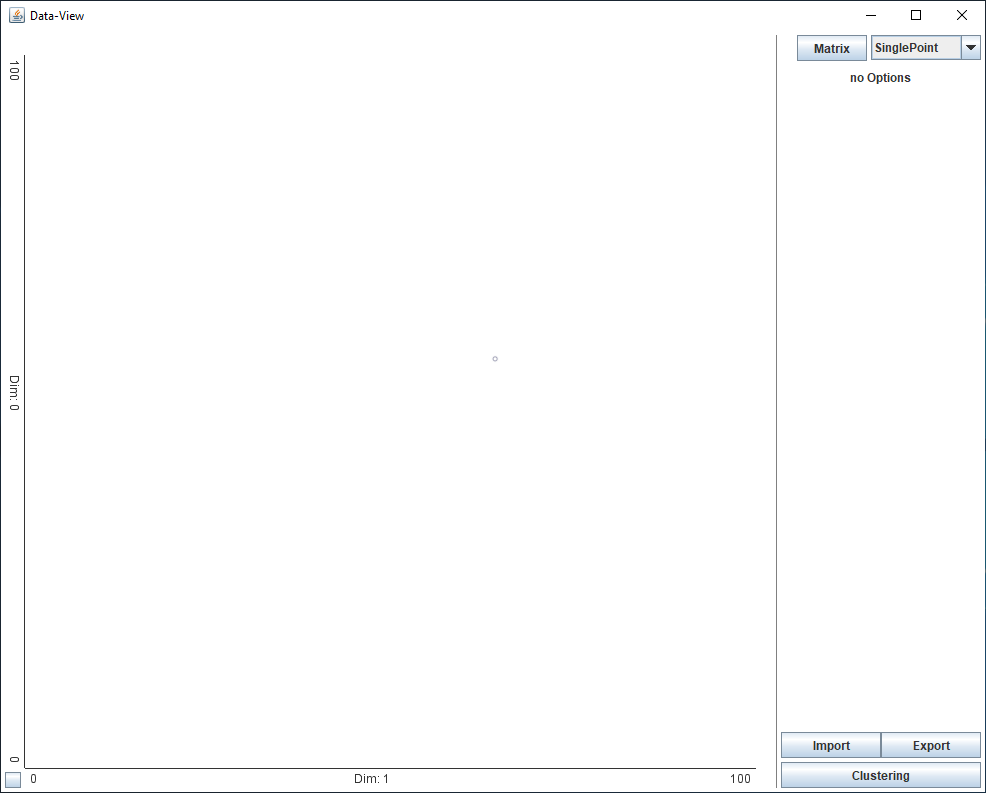
\includegraphics[scale=.45]{data-view}
	\caption{Data-View, the starting window of the application}
	\label{fig:data-view}
\end{figure}

\subsection{Plots and I/O}\label{sec:plotio}

The scatter plot in the center-left shows data that was imported or created and allows for changing the shown dimensions by clicking on the center of the corresponding axis. The range of values may also be adjusted this way, clicking on the upper or lower bound of the range on any axis opens a small input box. To automatically set this range, such that the minimum and maximum values of the shown data are just at the border, the small square button in the bottom-left can be clicked. This is also a useful feature for returning to a full view of the data if the range was made smaller to have a zoomed view of the data. The right part of the tool contains the functionality for importing/exporting data, manipulating the data, showing it in a scatter plot matrix and opening the workflow-view which will be explained in the next step.

 Firstly, to import a data-set for visualization and later use the import button in the bottom-right can be selected, opening a file dialog which can load either CSV or ARFF files. These formats are supported as they are most commonly used to store such data. This file dialog can be seen in Figure \ref{fig:data-import}. 

\begin{figure}[h]
	\centering 
	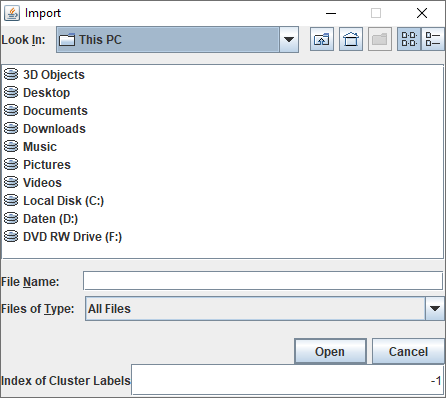
\includegraphics[scale=.45]{data-import}%[width=.5\textwidth]
	\caption{Import Dialog}
	\label{fig:data-import}
\end{figure}

After selecting a file the index of cluster labels can be defined if labels should be loaded from the file. Otherwise, the value can be left at $-1$ indicating that no columns should be used for label information. ``$-2$'' may be also be specified, it is used as a shortcut for selecting the last column as cluster label information, removing the need to count columns if it is the last one. The chosen column is then not inserted as a dimension in the data space but used only for the cluster labels, which the color of the loaded points will reflect in the scatter plot of the data-view. In Figure \ref{fig:loaded-data}, one can see how the data-view looks when data with cluster labels is shown. The data-set used for this example is the same as in Section \ref{sec:unob}.

\begin{figure}[H]
	\centering
	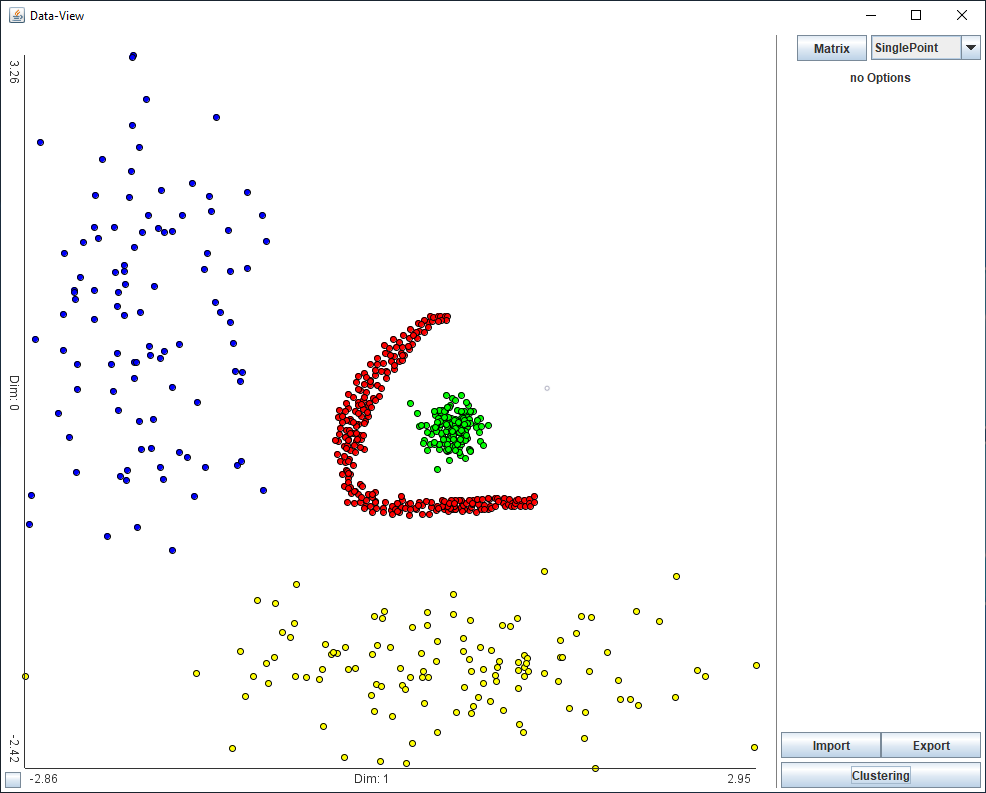
\includegraphics[scale=.45]{unob}
	\caption{Data-View with example data-set (including cluster labels)}
	\label{fig:loaded-data}
\end{figure}

To export data, the export button can be used. This button will open a similar dialog as for importing, though the index of the labels does not need to be defined, as data with cluster labels will be stored such that the labels for all points will be included in the first column. If the data does not contain label information, this first column is completely omitted. The supported format for exporting data is CSV.

Alternatively to importing, the user can also create a data-set himself from within the tool. It is possible to draw points onto the canvas when the ``SinglePoint'' option is selected in the top-right, as in Figure \ref{fig:data-view}. For this, the user only needs to click on the position of the canvas where he wants points placed. It is important to note that if there are more than two dimensions all values for the not shown dimensions will not be set, which may cause a problem for the clustering algorithms later on. Another possibility is the use of the ``ELKIGenerator'', which accepts an XML-style input for defining how to generate data. The definition for this format can be found in corresponding definitions file on the ELKI Github repository \cite{elkixml} or in the tools lib folder. This generator allows defining distributions on dimensions, the number of points for each generated distribution and many additional options like plane rotations. This can be quite useful when wanting to work with a quick sample data-set. 

In the top-right, the ``Matrix'' button can be used to display all dimensions at once, as it will open a new window showing the current data in a scatter plot matrix. Each scatter plot visualizes a different combination of dimensions and since the plots on the diagonal of this view are not useful, they were replaced with kernel density estimation plots. These kernel density estimation plots show how the values of the points in the corresponding dimension are distributed, overlapping the total distribution with the distribution of points with different labels. This may also allow seeing how clusters differ in each dimension. 

An example for this view can be seen in Figure \ref{fig:scatter_matrix} with the data-set from Figure \ref{fig:loaded-data}. Here, the kernel density estimations also already show a quite clear structure for the yellow and the blue cluster as each of those clusters nicely shows a Gaussian distribution in one dimension.

\begin{figure}[h]
	\centering
	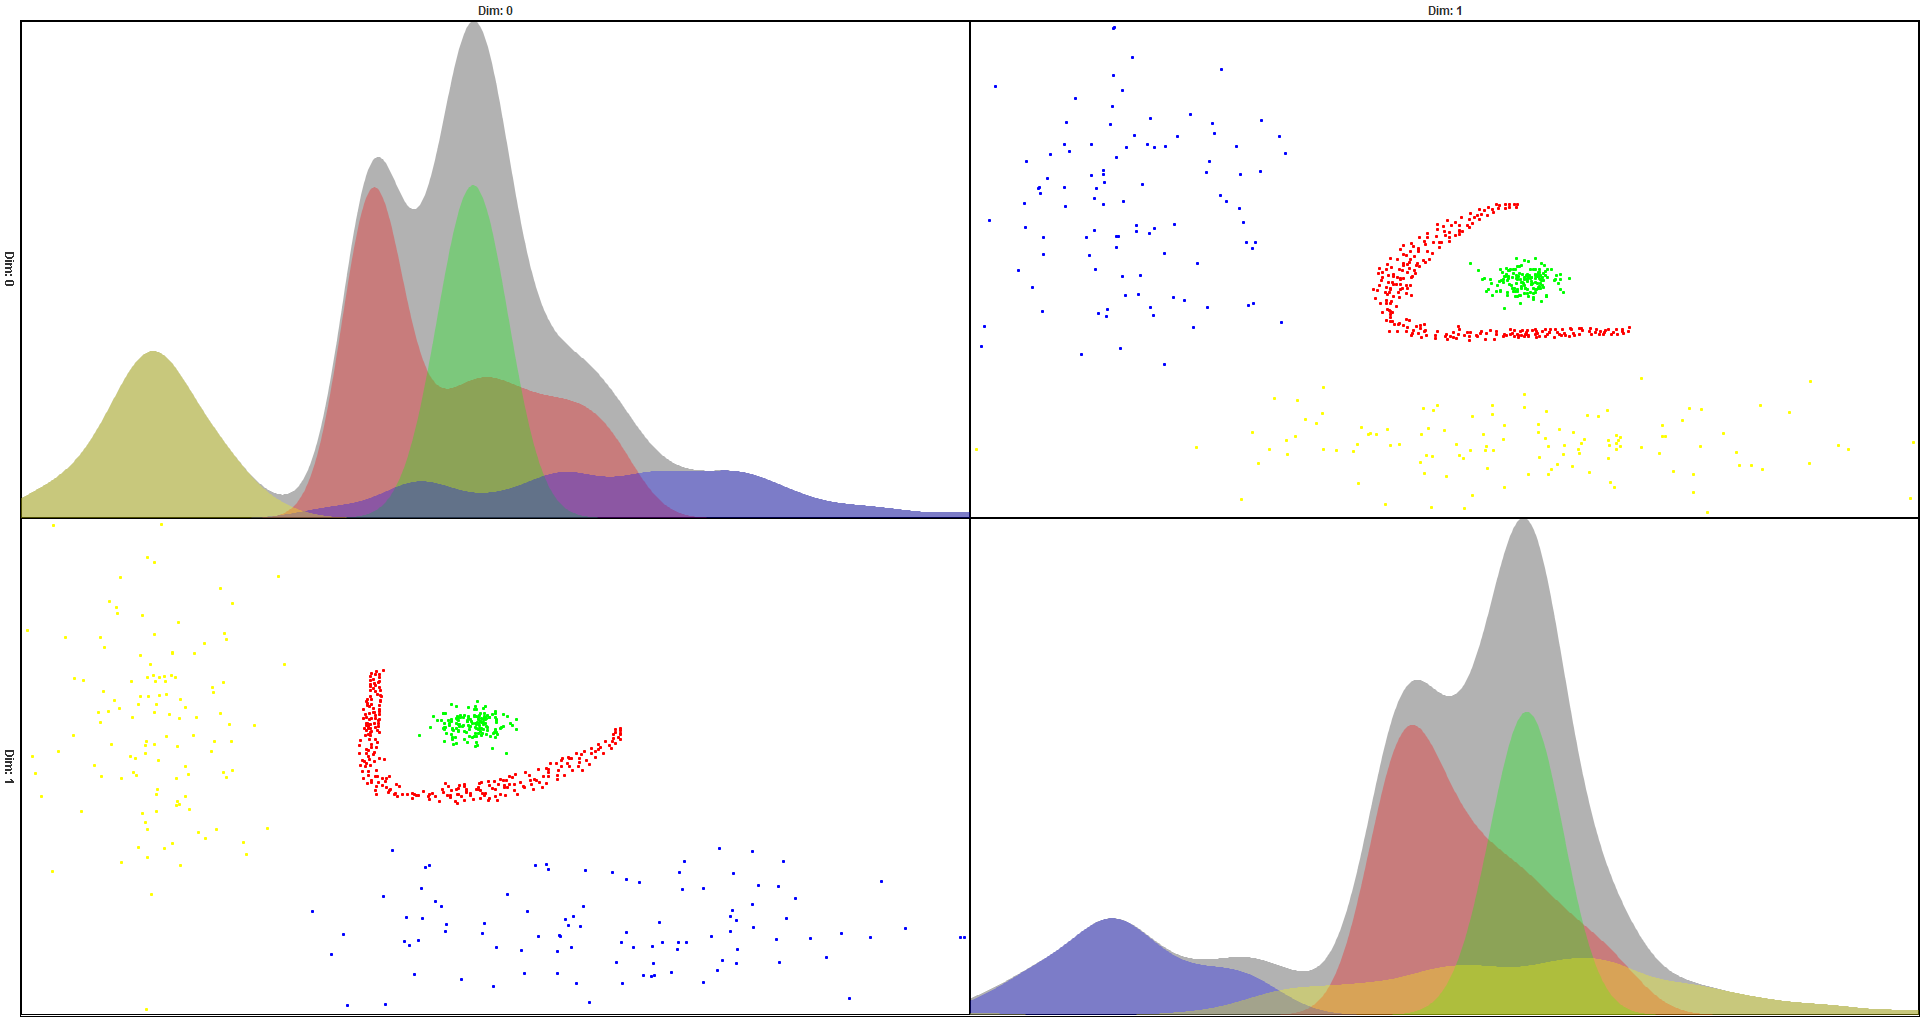
\includegraphics[scale=.25]{scatter_matrix}
	\caption{Scatter Plot Matrix for data-set from Figure \ref{fig:loaded-data}}
	\label{fig:scatter_matrix}
\end{figure}

\subsection{Modifying the data}

As the data may still contain unwanted dimensions after loading, cleanup may need to be done. To reduce the dimensionality, the simplest method is to select the ``Dim. Remover'' tool in the top right and define the index of the dimension to be removed. This tool may be a fitting choice when one knows that there is no or only little relevant information in a column. As more sophisticated methods Principal Component Analysis (PCA) \cite{pca} and t-Distributed Stochastic Neighbor Embedding (t-SNE) \cite{Maaten2008VisualizingDU} are also available. With these methods as much information as possible is tried to be maintained while reducing the dimensionality. PCA does this by calculating the principal components of the data and projecting it onto the $k$ strongest ones resulting in a reduced data-set with $k$ dimensions. $k$ can easily be defined in the settings of PCA by filling in the dimensions field. t-SNE works similarly to PCA, has more options though and even a parallel implementation. For more information on those methods see Section \ref{sec:dim_reduction}.

Other than reducing the dimensionality of the data, the application allows for normalization, such that it can be more easily used for clustering. If there are different dimensions with a strongly different meaning and range, this normalization step can benefit the accuracy of clustering greatly \cite{normalization}. The available tools are ``Normalize'' and ``Standardize''. Normalize changes the value range for each dimension to the interval $[0,1]$ while preserving relative distances, the Standardize tool adapts these ranges such that the average is $0$ and the standard deviation is $1$.

With the pre-processing done, the actual clustering of the data can be thought of next. To work on this next step the ``Clustering'' button can be pressed, opening the next major view of the tool.

\section{Selection of Algorithms and Parameters}\label{sec:sel_alg_param}
By clicking the ``Clustering'' button in the data-view, the window for managing clustering workflows, further on called workflow-view, opens. Here, clustering algorithms, their parameters and the parameters for meta-clustering can be defined. The workflow-view can be seen in Figure \ref{fig:workflow-view}, there no clustering tasks are added yet and all settings are set to their default values.

\begin{figure}[h]
	\centering
	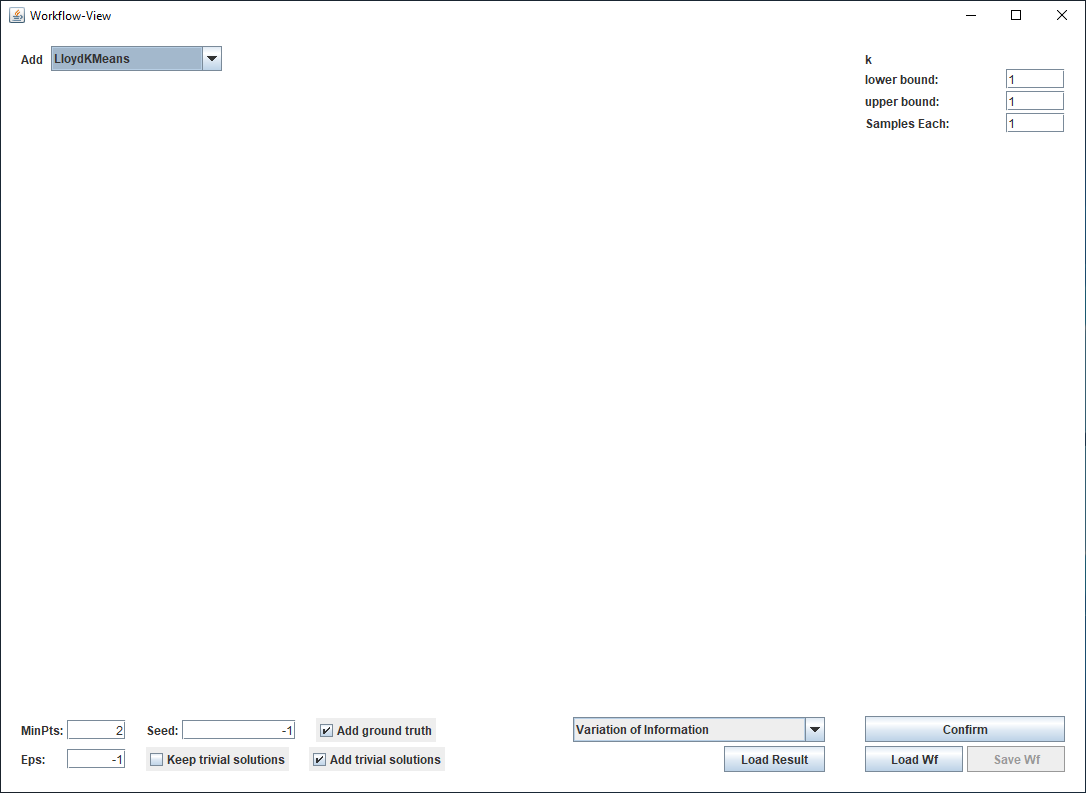
\includegraphics[scale=.43]{workflow-view}
	\caption{Workflow-View with no tasks and default values}
	\label{fig:workflow-view}
\end{figure}

In the top-left, the selector allows for choosing clustering algorithms to add to the workflow. When an algorithm is selected the corresponding options panel appears in the right allowing to set the parameter ranges that should be sampled. For each parameter the values used for clustering are drawn from a uniform distribution for each run, the number of runs can be defined in the ``Samples'' field. For some algorithms, where there is only the parameter for the number of clusters $k$, as for k-Means, the ``Samples Each'' setting defines how many runs to perform for each value within the range, instead of the total number of samples. This is the case as for such methods randomly sampling $k$ is usually not desired, only running the algorithm multiple times for each $k$, as random factors may impact the result. When all parameter ranges and the number of samples are defined, the clustering task can be added to the workflow with the ``Confirm'' button in the bottom right. If a clustering task should be removed, the ``X'' button beside the task can be clicked. An example of the workflow-view with defined clustering tasks can be seen in Figure \ref{fig:workflow-view-tasks}.

\begin{figure}[h]
	\centering
	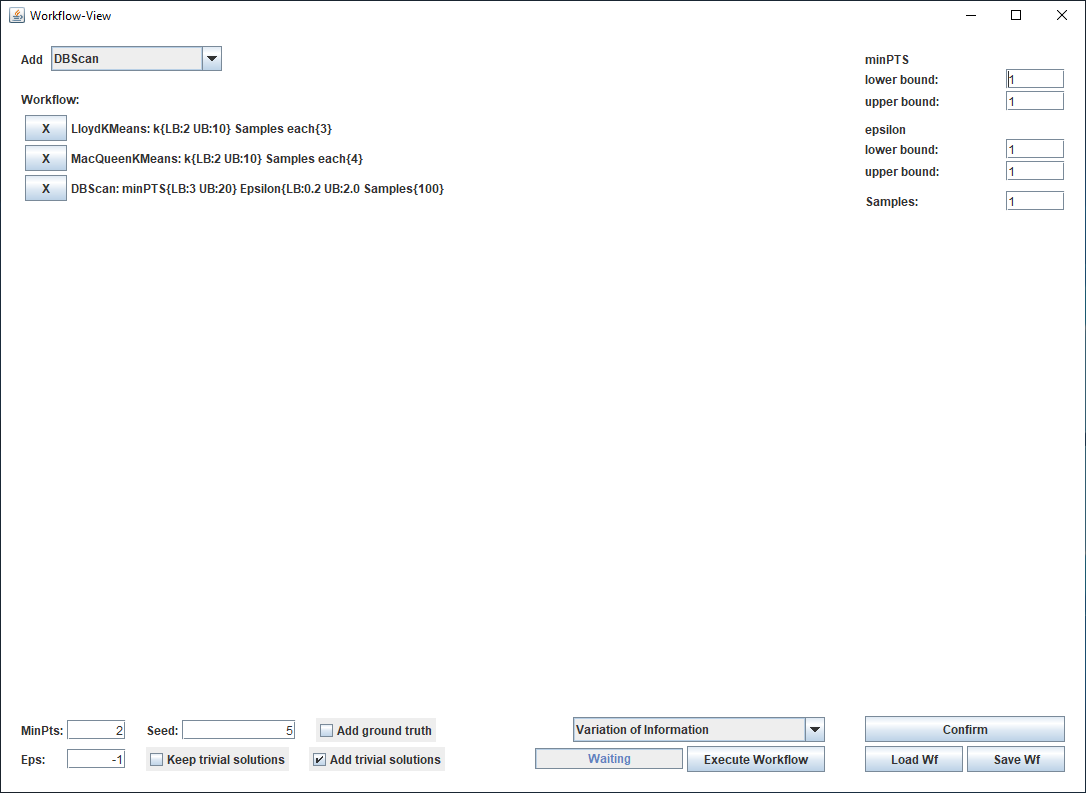
\includegraphics[scale=.43]{workflow-view-tasks}
	\caption{Workflow-View with tasks defined}
	\label{fig:workflow-view-tasks}
\end{figure}

For ease of use, workflows can be saved and loaded in the workflow-view, using the ``Save Wf'' and ``Load Wf'' buttons respectively. The tool creates custom Clustering Workflow Files (CWF) for this, allowing to re-use and modify workflows throughout multiple executions of the tool. This can be especially useful when working with standardized data-sets, such that the parameter ranges are similar or whenever k-Means is sampled. As this file does not depend on or reference a specific data-set, it may be used for different ones.

\begin{figure}[h]
	\centering
	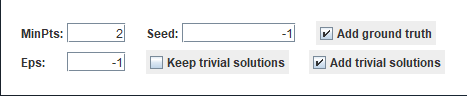
\includegraphics[scale=.75]{workflow-options}
	\caption{Options for setting Seed and OPTICS parameters}
	\label{fig:workflow-options}
\end{figure}

In the bottom-left, see Figure \ref{fig:workflow-options}, additional options are available which are not saved in the CWF files as the user should set them manually. Defining a random seed by setting the value for ``Seed'' to something other than $-1$ fixes the randomness of the clustering algorithms such that re-running them produces the same result every time, making results reproducible. For meta-clustering the OPTICS \cite{10.1145/304181.304187} algorithm is used as it produces a useful reachability plot in the meta-view, allowing for the identification of dense result regions which should indicate robustness of results. The ``Epsilon'' and ``MinPTS'' fields allow setting the parameters for the OPTICS algorithm, making it possible to define how close clustering results must be to be considered reachable and how many points need to be in this range. With these options, the user is able to define how densely related clustering results must occur for them to be shown as robust in the meta-view. The default parameters are chosen such that clusterings are always considered reachable and the neighborhood only considers the closest neighbor for reachability, leading to a processing order and result similar to single-link clustering. To select the distance function used by OPTICS, the selector in the bottom right just above ``Execute Workflow'' can be used. The ``Execute Workflow'' button is available as soon as at least one clustering task is added, as it replaces the ``Load Result'' button.

The additional checkboxes in the bottom-left allow adding the ground truth to the meta-view (if available) and to manage trivial solutions. Trivial solutions are in this case the solutions in which either all points were clustered into one cluster or each point was assigned its own cluster. One can delete trivial solutions occurring from the clustering algorithms or forcefully add them to the result, which may be visually helpful in the reachability plot later. These trivial solutions might also prove useful when comparing the NMI value of other solutions to the ground truth, to be able to compare how good their value is.

When all settings are defined, the user can press the ``Execute Workflow'' button, as visible in Figure \ref{fig:workflow-view}, launching a task that runs the algorithms and opens the meta-view with the computed results. In this step, the meta-clustering with OPTICS \cite{10.1145/304181.304187} is also performed.

If the user has a previously saved Clustering Result File (CRF), which can be created in the meta-view, he can also omit defining a workflow and load the results in through the ``Load Result'' button. This button is only available when no clustering tasks were added to the workflow, as can be seen in Figure \ref{fig:workflow-view-tasks}. Before loading a result though, the user should make sure that the settings in the bottom-left for meta-clustering are set to his liking. Only the seed field has no effect when loading a result as no clustering algorithms, except for meta-clustering which is deterministic, are run. After the data is loaded and meta-clustering is performed the meta-view again opens with the chosen data.

During the computation of the clustering algorithms and the meta-clustering, the loading bar next to the ``Execute Workflow'' button is updated, showing the current progress of the calculation.

\section{Meta-View and Consensus Clustering}
With either a clustering result loaded in or clustering algorithms run and the meta-clustering performed the meta-view is shown. Here, the terms `` clustering results'' and ``base clusterings'' are used interchangeably.

This view allows the user to comparatively explore the clustering results and thereby analyze their robustness. This should empower him in making educated choices on which clustering to pick as the final result or deciding on which ones should be combined into a consensus result. The meta-view can be seen in Figure \ref{fig:meta-view}, where example data is loaded and the ground truth is currently shown.

\begin{figure}[H]
	\centering
	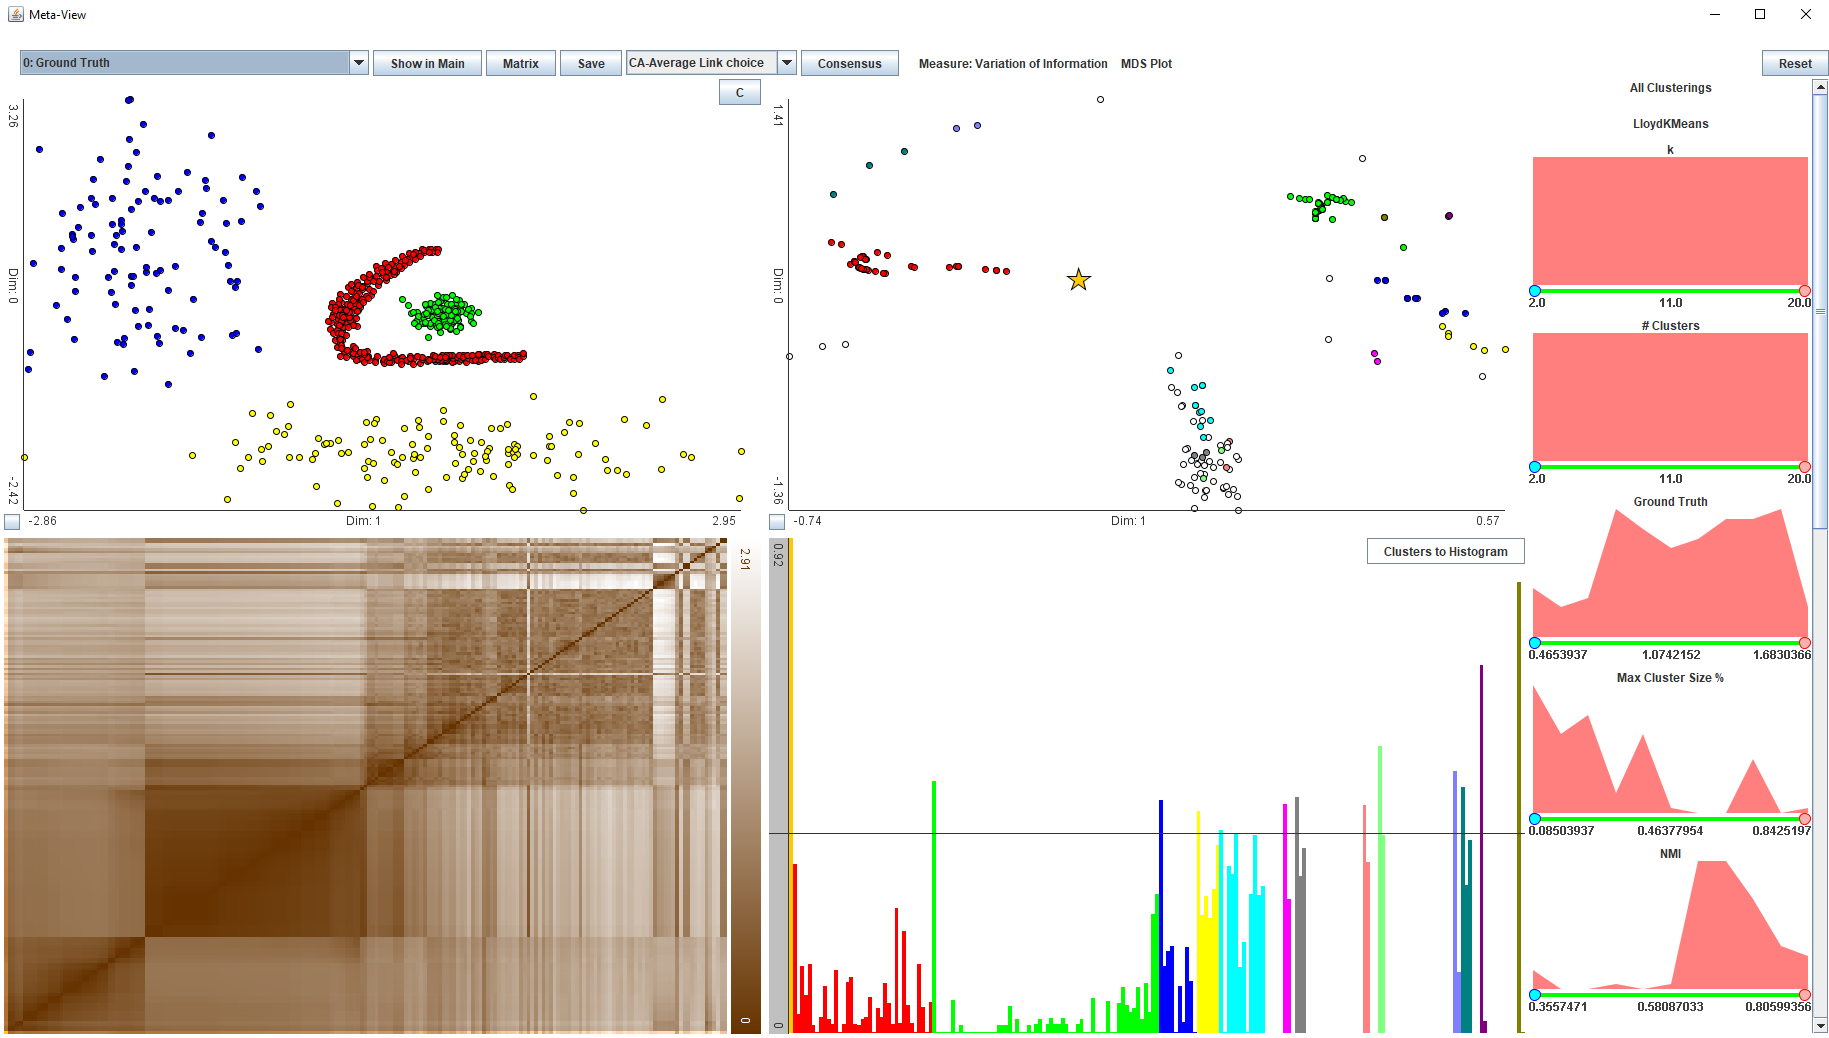
\includegraphics[angle=-90,origin=c,scale=.42]{meta-view}
	\caption{Meta-View with data and ground truth selected}
	\label{fig:meta-view}
\end{figure}

The meta-view consists of five main visual elements and some UI-elements at the top. Of the five elements, the left four visualizations give an overview of the data on an individual clustering and meta-level and the right part can be used to filter the base clusterings and look at area charts for different parameters. 

In the top-left visualization, the data can be seen with the points colored according to their cluster labels found in the result of the currently selected clustering run. The selected clustering can be changed by either selecting another one in the selector above or by clicking on a result in one of the other three views, that show them on a meta-level. When changing between selected clustering solutions, the colors for the labels are adapted such that the change of labels is minimal. This is done so the user can more easily see differences and is computed solving the mathematical assignment problem with Kuhn’s Hungarian method \cite{Kuhn2010}. If the user wishes to reset the colors for the labels of the currently selected coloring, for example when the recoloring leads to similar colors, he can press the ``C'' button in the top-right of the view, setting the colors back to their default values.

Above this scatter plot the ``Show in Main'' button allows the user to load the currently selected clustering back into the data-view, which can for example be useful if dimensionality reduction should be applied. The ``Matrix'' button opens the scatter plot matrix for the current clustering, this is the same visualization as when opened from the data-view. The ``Save'' button enables the saving of all clustering results at once using the custom Clustering Result File (CRF) format, as mentioned in the description of the workflow-view. This file can be loaded again from the workflow-view later. Alternatively, if only one clustering is selected, the CSV file type can be chosen and only the chosen clustering can be saved.

\begin{figure}[h]
	\centering
	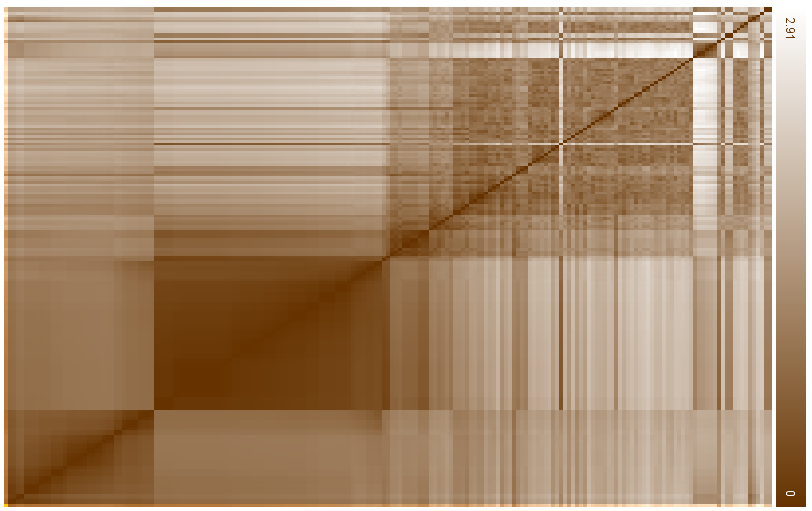
\includegraphics[scale=.45]{heat-map}
	\caption{Heat Map of the clusterings in Meta-View}
	\label{fig:heatmap}
\end{figure}

The bottom-left of the four visualizations shows a heat map representing the distances between clustering solutions, indicating hierarchical similarities when looking for dark-colored (i.e. dense) blocks on the diagonal. Figure \ref{fig:heatmap} shows such a heat map and one can see that depending on what the user considers to be a block, groups can visually be identified. The distances values plotted represent the ones calculated with the distance measure selected in the workflow-view and are color-coded such that their values can easily be compared in modulus. Clicking within this plot highlights the clustering corresponding to the column selected as well as the horizontal and vertical distance entries of the matrix. This should allow more easily analyzing distances between clusterings or clustering blocks within the matrix visually when adding them to the selection through control-clicking. Whenever a single clustering is selected it is also shown in the top-left and any selection is also updated to the remaining views in the meta-view.

\begin{figure}[h]
	\centering
	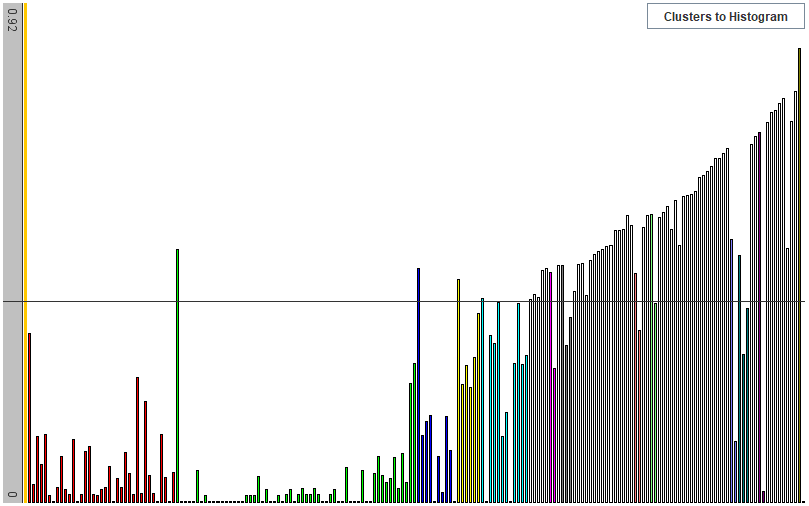
\includegraphics[scale=.45]{reach-plot}
	\caption{OPTICS Reachability Plot in Meta-View }
	\label{fig:opticsplot}
\end{figure}

In the bottom-right, the reachability plot resulting from the OPTICS meta-clustering is shown, it can be seen in Figure \ref{fig:opticsplot}. The height of each individual bar represents the reachability value for the clustering as determined by the algorithm and valleys in this plot can be interpreted as clusters. For more information on the reachability value, refer to Section \ref{sec:opticstheory}. To define the meta-clusters the gray range bar can be clicked or dragged on, moving the threshold line. With the threshold defined the clusterings are colored according to the meta-cluster they belong to, a meta-cluster is found whenever the line intersections with the bars find valleys. Also, clicking or control-clicking on bars modifies the selected clustering(s), again updating the other views. If ground truth is available, mousing over the bars shows a tooltip with the distance and the NMI of the clustering in relation to the truth. With the meta-clustering defined, double-clicking on a bar or point in any other plot on the meta-level will select the whole meta-cluster. This chart can also be used as help for deciding on which clustering to pick for the final result as neighboring bars with small values indicate a dense region of results. Such a dense region can be interpreted as a robust solution and choosing a clustering from it may yield a good final choice. 

In the top-right of the reachability plot the button ``Clusters to Histogram'' allows the user to only show clusterings in the filter panel and its area charts which are assigned to a cluster. This leaves out the noise and allows for seeing the parameter distributions of the deemed robust clusterings, such that filtering is facilitated. To undo this, the ``Reset'' button above the filter panel can be clicked, both resetting all filters and showing all clusterings in the area charts of the panel.

\begin{figure}[h]
	\centering
	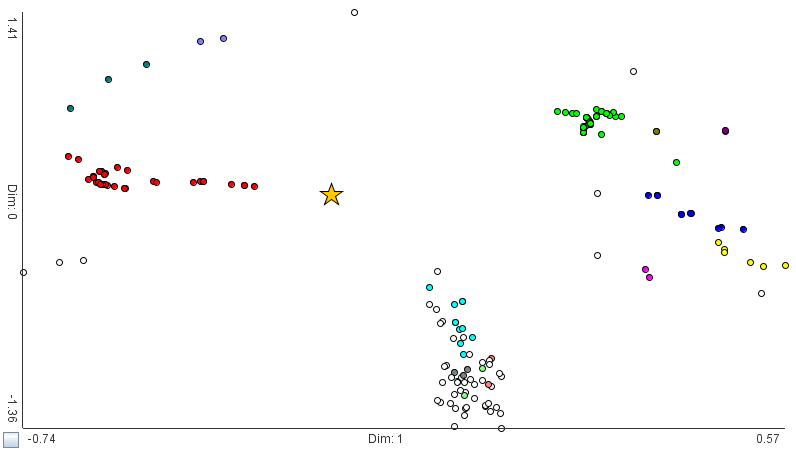
\includegraphics[scale=.45]{mds-plot}
	\caption{MDS Plot in Meta-View}
	\label{fig:mdsplot}
\end{figure}

Above the reachability plot, in the top-right the MDS plot is visible, it can be seen in Figure \ref{fig:mdsplot}. This visualization shows an approximate representation of the clusterings as points in a finite-dimensional space, aiming to stay as true as possible to the distance between them. The computation of this representation uses Multi-Dimensional Scaling (MDS) \cite{mds} which also gives this plot its name. When ground truth is available, it is shown in this plot as a star and the other clusterings are colored according to the threshold set in the OPTICS plot. This visualization is useful as the user can, similarly to the heat map, explore which clusterings are close to each other and where the ground truth lies in this representation space. An ideal sampling of the solution space could be claimed if the ground truth is central, as the represented space approximates the solution space. With many clusterings surrounding the ground truth, consensus clustering is also more likely to find a result close to the ground truth, as its goal of combining clusterings aims to find a result in the center of the solution space spanned by the clusterings. In the MDS plot, the user can also once again select points by clicking. Additionally, dragging and selecting multiple points at once is possible here as well. Besides this, all functionality available in simple scatter plots can also be used here, e.g. editing the range of shown values.

\begin{figure}[h]
	\centering
	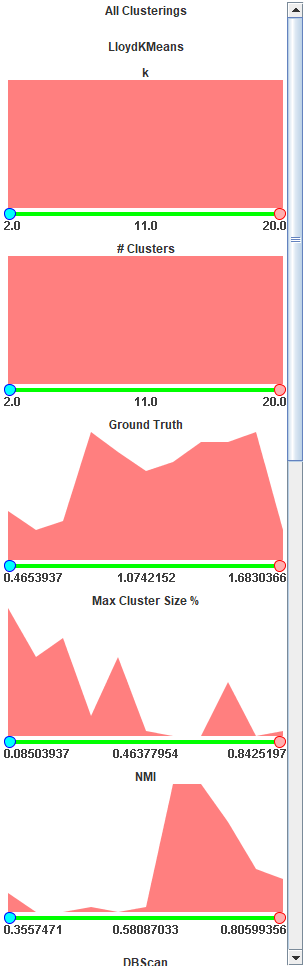
\includegraphics[scale=.5]{filter-panel}
	\caption{Filter Panel in Meta-View}
	\label{fig:filterpanel}
\end{figure}

In the very right of the meta-view the filter panel can be seen, as depicted in Figure \ref{fig:filterpanel}. There, clusterings can be filtered such that they are less visually prominent in the other views and won't be used for consensus calculation. To define which clusterings to filter out, the user can drag the range bars below each area plot, reducing the range of values for a clustering to be considered relevant. The area charts above these bars depict how many clusterings have approximately which value and how many of them were filtered out (in blue) in comparison to how many weren't (in red). Also, note that either all clusterings are visualized in these area charts or only the ones that were assigned a meta-cluster if the ``Clusters to Histogram'' button was pressed above the reachability plot.

Next to the ``Save'' button in the top row, a consensus function can be chosen in the selector and used by pressing the ``Consensus'' button, see Figure \ref{fig:cons_button}. 

\begin{figure}[h]
	\centering
	
\includegraphics[scale=.75]{cons_button}
	\caption{Buttons in the top of the Meta-View}
	\label{fig:cons_button}
\end{figure}

When this button is pressed, a dialog window opens if the consensus function supports defining the number of clusters in the result. With this, the user can define this parameter to force this number of clusters or leave this field empty when the function should try to estimate this parameter itself (Figure \ref{fig:choosek_window}).

\begin{figure}[h]
	\centering
	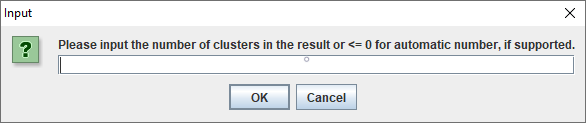
\includegraphics[scale=.6]{choosek_window}
	\caption{Input for Number of target Clusters for Consensus}
	\label{fig:choosek_window}
\end{figure}

The consensus function then aims to combine the clusterings belonging to the same meta-cluster, ignoring the ones filtered out as well as the ground truth if available. When the calculation is done, a new meta-view opens using the consensus results as data. This new view will contain as many clusterings as there were meta-clusters in the previous view and, if it was available, the ground truth in the first position.

The selection of the final result can be done by either searching for robust solutions in the visualizations of the meta-view or by performing consensus clustering, merging all clusterings or groups of robust solutions. When consensus clustering is used, additional knowledge can be gained from other solutions and the overall result may be better than any individual run, though the consensus results may be more difficult to interpret.

\chapter{Implementation}\label{cha:impl}
\section{Programming Language and Tools}
For the implementation of my tool, my language of choice was Java. With Java, there are lots of available implementations for different clustering methods, including the Frameworks ELKI \cite{10.1007/978-3-540-69497-7_41} and WEKA \cite{10.1145/1656274.1656278}, as well as the machine learning library Smile \cite{javasmile}. 

To improve the performance in some parts of the tool Java 1.8 was chosen, making it the lowest required Java version to run it. This was done, as it enables the use of parallel streams which make it simple to parallelize loops with independent iterations. Additionally, it is easy to create custom visualizations using the low-level draw() method of JComponents in Swing \cite{javaswing}. All graphs and plots were created using a custom draw() method as this also leads to much better performance than using many small components for the plots.

\section{File Input and Output}
Loading and saving data is needed for the tool to make it more usable. For this reason, it is possible to not only import data for clustering but also to save workflows and whole groups of clustering results for later reuse.
\subsection{Clustering and Point Data}
Besides being able to create new data sets from within the tool, importing data from CSV or ARFF files is possible. Those file types are supported as they are very common, especially CSV is usually used to store such information. ARFF is commonly used, as it is also the preferred data type of WEKA \cite{10.1145/1656274.1656278}. For this reason, the ARFF importer of WEKA was adapted to load in these files such that they can be used with this tool. 

When importing data, it is also possible to define an index of where the cluster labels are located. When this is done the tool will not load the specified column as data but use it to define clusters for the ground truth, which is then also handled differently by the different views of the tool.

The starting window or data-view, in which clusterings can also be loaded back into from the meta-view, also allows for exporting data to CSV. When doing this, the first column in the resulting file will contain the cluster identifiers starting with one. This way computed results can be exported and used in other tools or saved for later.

\subsection{Clustering Workflows}
As many runs of clustering algorithms with different parameter ranges can be performed and repeatedly defining this workflow can be tedious, the tool allows exporting and importing these workflows from the cluster workflow window. For this, the underlying clustering objects are serialized and saved into .CWF (Cluster Workflow Files). It is important to note, that these files do not include the parameter settings for random seed or meta-clustering. This is intentional as I do not consider them to be part of the workflow and they should be set by the user for every run if the default values are not satisfactory.

\subsection{Pre-Clustered Data}
Due to the clustering algorithms possibly being time-consuming, either because of their complexity or just the sheer number of runs, the results of these algorithms can be saved from the meta-view. To do this, the clustering result objects are serialized and saved as .CRF (Clustering Result Files). To load those files one can define the different parameters of the meta-clustering and then import the .CRF. This way, only the meta-clustering is computed again. The meta-clustering is not saved in this file such that the user can more easily try different settings for it, by just saving the result and running the meta-clustering again. As this is usually much faster than the clustering algorithms that generate the base clusterings, saving the solutions may save a considerable amount of time.

\section{Methods and Interfaces}
To ensure that new or missing methods can easily be added to the tool, all methods where a selection can be made from within the tool can be added to by implementing onto the corresponding interface. To add a method one needs to first implement it and if needed it's OptionsPanel, then adding it to the corresponding static method found in the view using it.

The following sections describe which interfaces and standard methods are implemented, as well as which functions and classes must be edited to add new custom methods.

\subsection{Data Manipulation}

Data manipulation can be performed as a first step in the data-view to create data-sets or modify them such that they can be used for clustering or visualization. It is also of relevance when loading clustering results back into the data-view to analyze results using dimensionality reduction techniques. For this, step three interfaces are of interest:

\begin{itemize}
  \item Generators: IGenerator
  \item Reducers: IReducer
  \item Normalizers: INormalizer
\end{itemize}

%maybe show interface definitions?
\subsubsection{Generators}
Generators allow the user to add or replace data points. Two initial implementations for generators are available, firstly the SinglePointGenerator which allows adding points to the data by clicking the scatter plot. When a point is added this way its coordinates are set to where the user clicked on the screen translated into the coordinates of the data space, such that the point appears below the cursor. Secondly, the ELKIGenerator is available which uses an XML-style input, defining how the clusters should be generated. This class uses the GeneratorXMLDatabaseConnection of ELKI \cite{10.1007/978-3-540-69497-7_41} and is able to create data points according to different random distributions. The definitions file for this input can be found in ELKI's JAR file, their GIT repository \cite{elkixml} or in the /lib folder of the implementation.

%implement SamplingReducer?
\subsubsection{Reducers}
Reducers allow the user to manipulate the data such that the dimensionality or potentially (in the future) the number of points can be reduced. Per default three dimensionality reduction techniques are available. The simplest one, DimensionRemover, enables the user to just define a dimension by its index and delete it. This can be useful if the data is not well cleaned beforehand and irrelevant or possibly disrupting columns are present in the data. For more advanced dimensionality reduction, the PCAReducer and tSNEReducer are available. The PCAReducer, which is adapted from the implementation from Smile \cite{javasmile} uses Principal Component Analysis \cite{pca} to reduce the dimensionality of the data to what the user-defined. In contrast, the tSNEReducer adapted from Jonsson \cite{javatsne} uses t-Distributed Stochastic Neighbor Embedding \cite{Maaten2008VisualizingDU} and also requires a perplexity parameter.
%perplexity???????

\subsubsection{Normalizers}
Normalizers provide functionality for normalizing the data points. This may be useful whenever different dimensions contain values in strongly differing ranges, while their concrete values do not have any direct relation to the other dimensions \cite{normalization}. Here, two default implementations are available, Normalize and Standardize. The Normalize class adapts the values such that in each dimension the range is set to the interval $[0,1]$ while preserving relative distances. The Standardize class adapts these ranges such that the average is $0$ and the standard deviation is $1$.

\subsubsection*{Adding Data Manipulation Methods}
To add additional Methods they must be implemented using the corresponding interface and added to the class DataView. To add them to this class the static methods initGenerators(), initReducers() and initNormalizers() must add the new method to the list of methods. As an example adding a new generator (newGeneratorX) would require adding ``generators.add(new newGeneratorX());'' to the function initGenerators().

\subsection{Clustering Algorithms}
Clustering algorithms can be selected and tuned in the clustering workflow window such that the algorithm is used to create base clustering results for the meta-view. For additional information on the algorithms themselves, see Section \ref{theory_clustering}. The following interfaces are relevant for clustering:

\begin{itemize}
  \item Clustering Algorithms: IClusterer
  \item ELKI Clustering Algorithms: IELKIClusterer
  \item Custom Clustering Algorithms: ICustomClusterer
\end{itemize}

\subsubsection{Clustering Algorithms}
Clustering algorithms can be used in the workflow-view to generate base clusterings for meta-clustering and visualization in the meta-view. The interface IClusterer is used as a helper interface such that all clustering algorithms can use the same high-level calls for compatibility. The actual implementations implement either IELKIClusterer if they use the ELKI database objects in their logic or ICustomClusterer if they use a data matrix. To further help adding methods by not needing to re-implement generally needed functionality, the class AbstractClustering should also be extended by the actual implementation. With this abstract class and the interfaces the actual implementations can focus more on just the clustering logic. Additionally, options panels should be created for each new algorithm allowing the user to set parameters or parameter ranges from the tool.

\subsubsection{ELKI Clustering Algorithms}
IELKIClusterer is used for clustering algorithms that use ELKI's database object to store the data. To run algorithms from ELKI this interface must be implemented and the database object can be used with ELKI's algorithms. The pre-implemented methods include three variants of KMeans, DBScan and EM clustering. All of these methods use ELKI's high-level initialization with ``ClassGenericsUtil.parameterizeOrAbort(AlgorithmClass.class, params);'' and other than this only require the logic for managing parameters, random sampling and collection of the result.

\subsubsection{Custom Clustering Algorithms}
To enable other clustering algorithms than the ones implemented in ELKI the interface ICustomClusterer can be used. It receives the two-dimensional data array and the headers as input and allows for the use of any custom clustering logic. One implementation is already available here, namely Spectral Clustering which is implemented with the Smile library \cite{javasmile}.
 
\subsubsection*{Adding Clustering Algorithms}
To add new clustering algorithms for creating base clusterings, first one must choose IELKIClusterer if the method uses ELKI's database object or ICustomClusterer otherwise. This interface then needs to be extended, the AbstractClustering class can help here with utility functions. When extending the corresponding interface an options panel must be implemented and the parameters must be managed within the cluster() function. These interfaces also provide functionality for seeded randomness and progress indicators. To properly calculate progress, getCount() must return the proper number of needed executions and cluster() must call addProgress() whenever progress is made. Finally, the newly implemented class must be added to the initClusterers() function in ClusterWorkflow.


\subsection{Meta-Clustering}
%info on OPTICS?
The algorithm used for meta-clustering is OPTICS \cite{10.1145/304181.304187}. One of the requirements for these methods is that the used distance measure must be metric, otherwise the algorithm can only produce an approximate clustering at best. The distance measure used by the algorithm can be changed and additional distance measures can also be added. For this, the following interface is of interest:

\begin{itemize}
  \item Clustering Distance Measure: IMetaDistanceMeasure
\end{itemize}
\subsubsection{Clustering Distance Measures}
The interface IMetaDistanceMeasure is used to define distance measures that can be used for OPTICS for meta-clustering. These distance measures should represent how different two clustering solutions are from each other while needing to fulfill the requirements of a metric. For a distance measure, here indicated with $d(x,y)$ where $x$ and $y$ are objects, to be considered metric the following conditions must hold \cite{10.5555/1756006.1953024}:
\begin{itemize}
  \item $d(x,y)\geq0$: distances must be non-negative
  \item $d(x,y)=0$ iff $x=y$: the distance between two objects is zero if and only if both objects are equal
  \item $d(x,y)=d(x,y)$: the distance must fulfill the symmetry condition
  \item $d(x,z)\leq d(x,y)+d(y,z)$: the triangle inequality must hold
\end{itemize}

If the requirements of a metric are not fulfilled the measure can only be used as an estimate and may produce unsatisfying clusterings. The default implemented measures are Variation of Information and the Clustering Error. 

Variation of Information (VI) \cite{10.1007/978-3-540-45167-9_14} measures how much information is gained/lost when changing a clustering to another. It considers relationships between points and their clusters instead of the relationship between two points and is closely related to the mutual information measure. Unlike mutual information, VI is metric and can therefore be used as a distance measure here.

Clustering Error (or classification error) \cite{MEILA2007873} represents the fraction of misclassified points assuming one clustering represents the labels of the truth. To compute this the clusters first need to be mapped to one another such that maximum overlap is obtained in a confusion matrix, i.e. finding a permutation where diagonal entries are maximal. To do this Kuhn’s Hungarian method \cite{Kuhn2010} is used and the diagonal elements of the matrix are summed up. This gives us the number of points for which the two solutions agree, which is subtracted from the total number of points. The resulting value is then divided by the total number of points giving us the desired fraction.
%%%% metric????
%%%%https://publikationen.bibliothek.kit.edu/1000011477/812079

\subsubsection*{Adding Distance Measures}
To add distance measures for OPTICS the interface IMetaDistanceMeasure must be extended and the above-mentioned conditions on the distance measure must be fulfilled for the algorithm to produce a satisfying result. After implementing the distance function it must be added to initDistances() within ClusterWorkflow, such that it is usable from within the tool.

\subsection{Consensus Clustering}
Consensus Clustering can combine the results form different base clusterings into a common clustering. This can be done in the meta-view and different algorithms can be used for this step. When run, the algorithm computes a consensus result for all base clusterings that are in a common meta-cluster in the OPTICS reachability plot and are not filtered out. This means that if the user defined three meta-clusters with some cut-off value in the reachability plot, there will be three resulting consensus clusterings, one created from each group. The interface of interest for consensus functions is:

\begin{itemize}
  \item Consensus Functions: IConsensusFunction
\end{itemize}

\subsubsection{Consensus Functions}
The consensus functions implement the logic for combining the base clusterings. For this, the interface IConsensusFunction is of interest and can be extended to add new functions. Per default two main implementations are available. Both implementations allow for the user to either define a target value for the number of resulting clusters $k$ within each result, or for the algorithm to guess this parameter itself. Firstly, CoAssociationMatrixAverageLink can be used, which computes a Co-Association (CA) Matrix and combines objects via the average link strategy. When $k$ is defined the algorithm joins together sets of points until only $k$ sets remain, which is used as the final answer. If no $k$ is defined the algorithm performs two runs, calculating the lifetime \cite{lifetime} of the resulting tree and choosing the level to cut as the one resulting with maximum lifetime. As second method DICLENS is available, which was generously provided by Mimaroglu and Aksehirl \cite{DICLENS}. Parts of their implementation were modified to allow for parallelism whenever this was a simple change.

\subsubsection*{Adding Consensus Functions}
To add consensus functions the interface IConsensusFunction must be extended. It is also important to note that weights may be supported by the function if implemented, although at this point there is no way for the user to set weights. As for the two default implementations, the function may either allow defining the number of resulting clusters per consensus result or not. To add the newly created function to the tool, within MetaViewer the function initConsensusFunctions() must include the new method.

\section{Visualization}

To visualize the data in different ways and provide a functional Graphical User Interface (GUI) the Java Swing \cite{javaswing} Toolkit was used. It allows for both high-level calls creating objects (JComponents) within windows, e.g. panels, buttons or combo-boxes, as well as low-level calls by directly changing the behavior of the draw() function. For the basic GUI, the panels and buttons of the tool were created with high-level calls, while the different graphs and plots were implemented by overriding the draw() function. Overriding the draw() function immensely improved performance as the already available high-level objects are computationally costly by comparison when many of them are needed. This section only includes additional information on the implementation and functionality, information on the usage of the visual elements in the tool can be found in Chapter \ref{cha:Tool}.

\subsection{Scatter Plot}
The scatter plot is the simplest visualization of the data within the tool. It is implemented though two axis and a canvas object. The axis includes logic for the drawing the value range and selected dimension, the mouse listeners for modifying it, as well as the translation from model coordinates to viewer coordinates. The canvas implements the drawing of data points, including different shapes and colors depending on their cluster identifier, whether or not they are filtered out or if they represent special objects like the ground truth in the meta-view. Additionally, the canvas can support mouse listeners enabling interactivity with the points.
%more?

\subsection{Switching between Clusterings}

In the meta-view, the user is able to change the currently visible clustering by selecting another clustering in the drop-down menu, the heat map or the reachability plot. Whenever this happens the scatter plot showing the current clustering is exchanged and replaces with one showing the selected data. As the labels may be totally different and comparing them in this switching process is visually difficult when they are assigned different colors, Kuhn’s Hungarian method \cite{Kuhn2010} is used to color the points of the newly shown clustering according to the previously shown one. This results in visually similar choices of color for points and thereby allowing for easier comparison. In the general case, this problem is called the mathematical assignment problem, which has many applications in different fields \cite{Kuhn2010}.

\subsection{Scatter Plot Matrix}

The scatter plot matrix implements a view that constructs a grid of scatter plots, one for each combination of dimensions in the data. For the elements on the diagonal of the grid, the plots are exchanged with kernel density estimation plots which are computed using the Java Smile \cite{javasmile} library. Kernel density estimation usually needs a bandwidth parameter to be set which influences how the resulting distributions look. The smile library implements a default value for this parameter though, which estimates a fitting value for this bandwidth. The plot then uses the maximum density for the whole data-set as the $100\% $ mark, drawing it up to the top of the grid cell. On top of this function, the functions representing the density for each cluster label are overlayed with different colors and some opacity such that they are all visible. These overlayed functions are assigned their height value by multiplying the density estimation value with the percentage part of the data they contain (e.g. cluster contains $5\% $ of data points $\rightarrow$ height times $0.05$) and scaling these values to screen coordinates, just like the overall function. This results in the function for the whole data representing the sum of the functions for each cluster label.

\subsection{OPTICS Plot}
The OPTICS reachability plot shows the clusterings with their computed reachability values computed by the OPTICS algorithm ordered according to their order in which they were processed. For additional information on OPTICS see Section \ref{sec:opticstheory}. Clicking or dragging on the gray range bar changes the threshold for which clusterings are considered to be in a meta-cluster and the colors are adapted accordingly. The colors of the clusterings, when represented in the MDS plot, are also defined through this threshold. The OPTICS plot, just like the heat map and the MDS plot allows for selecting clusterings through clicking or control-clicking on them, whenever multiple clusterings should be selected.

The implementation of the OPTICS algorithm, creating the data required for this visualization is based on the proposal of Ankerst et al. \cite{10.1145/304181.304187}, using a priority queue to efficiently keep a fitting order for the clusterings that need to be processed.

\subsection{Heat Map}
The heat map shows the distances between clustering solutions using the meta distance measure as defined by the user. It allows for visually identifying blocks of similar results on the diagonal, different hues of brown were chosen for this as they are easier to distinguish than other colors tested. The plot is drawn by overriding Java Swing's \cite{javaswing} draw() function, as creating a component for each cell makes the view unresponsive due to the large overhead from managing a large number of components. To allow for mouse interactivity the coordinates of clicks were calculated back to find the targeted cell and used for selection logic. This is needed as there are no small components, which would usually manage this.

\subsection{MDS Plot}
The Multi-Dimensional Scaling (MDS) plot shows points such that their actual distances are approximately represented in a fixed dimensional space. This is done with the equally named method multi-dimensional scaling, \cite{mds} for which a maximum number of dimensions $d$ must be defined and the input requires a distance matrix for the points to be layed out. This method is implemented using the Java Smile \cite{javasmile} library and trying to use as many dimensions as possible. With $d$ set, it aims to compute approximate coordinates for the points by trying to keep the distances in a $d$ dimensional space as true to the inserted distance matrix as possible. The resulting coordinates, similarly to PCA, also capture as much information as possible in the leading dimensions, resulting in the first two being the best choice to visualize in 2D. This is the case as MDS actually computes the same result as PCA whenever the distances are Euclidean. To show this information, the created points are loaded into a scatter plot and per default these first two dimensions are shown. Whenever more than two dimensions are available the user can change the shown dimensions by clicking on the corresponding axis and choosing another dimension. The selection of points can be done by either clicking or dragging on the canvas of the scatter plot. When clicking the closes point is selected and when dragging all points within the drawn rectangle are selected.

\subsection{Filter Panel}
The filter panel allows the user to filter out results by decreasing the range on the range selectors. The area charts show how much data points are within the range in red and how many points are outside it/filtered out in blue. This chart is implemented by defining buckets for the values to be shown and counting the number of value occurrences within each bucket. For double values the square root of the number of values is used as the number of buckets, for integer values the number of values in their range is chosen and for Boolean values 3 buckets are chosen. 3 buckets were chosen there, such that true is shown on the left, false on the right and there is space in the center for clearly separating the two values. If there would be too many buckets when using this default calculation they are capped at 31 (as uneven numbers may produce nicer ranges), which helps for example whenever too large integer ranges are available. Also, as the charts are quite small, more buckets can no longer be visualized properly.

For each clustering algorithm type a separate chart and range selector is created for each parameter and some additional filters are available. The parameters are found through the Parameter object which must be added to a clustering result by the class performing the clustering algorithm. The additional filters include the distance (as chosen by the user) to the ground truth and the Normalized Mutual Information (NMI) \cite{10.5555/1756006.1953024} whenever ground truth is available, as well as the ratio of the size of the largest cluster relative to the number of points. This ratio may be useful as clusterings where e.g. if more than $90\%$ of the points are within one cluster, the solution may not be satisfactory. More such filters can be added by providing the needed values to the clustering results through the addParameters() function in the MetaView class.

When the range is reduced, filtering out results, the other views are updated to reflect this change by changing the opacity of the corresponding points/cells.

\subsection{Cluster comparison}

For the comparison of two clustering results, it is possible to select two clusterings in the meta-view by control-clicking a second clustering when only one is selected. Whenever two clusterings are selected a ``Difference'' button appears, clicking it opens the comparison view. Here, just like when switching between visible clusterings, they are adapted with Kuhn’s Hungarian method \cite{Kuhn2010} such that their common labels are maximal. The center view then colors all points where the labels differ in black and the ones where they are equal in white. This allows to quickly see which points differ for solutions that are at least somewhat similar. The percentage of differing points shown in the title bar of this window is computed by dividing the number of black points by the total number of points.

\part{Testing}
\chapter{Experiments}\label{cha:experiments}
To show the value of the new tool, different scenarios created. The goals of the tool are to improve on the ease of finding complex cluster structures and improve on the result in comparison to only using simple clustering methods. Another aim is to visualize the data and clustering results such that an expert user can make a well-informed decision on which solutions best fit the data. For all experiments performed the Variation of Information distance measure was used, as it produced better results and the random seed was fixed at $1$ for reproducibility of the experiments. The parameters for OPTICS were also left at their default values, as more fine-grained valleys are visible. The default choice for $\epsilon$ also leads to a worse runtime for the algorithm, this is acceptable though as the clustering algorithms take more time anyways.

\section{Solutions better than Base-Clusterings}
To show that the tool is able to find better solutions than just the ones produced by single clustering runs, different examples are presented in the following sections. 
\subsubsection{k-Means}
Creating base clusterings and applying consensus functions are well-known methods, but there was previously no tool allowing to perform these steps as easily with a visual interface. Using this tool, a user is able to find better results than the individual ones created by sampling the parameters for the different clustering algorithms. This is the case as the combined knowledge through consensus clustering can be more powerful than an individual algorithm due to information from other results being ignored when deciding on a sampled solution.

\begin{figure}[h]
	\centering
	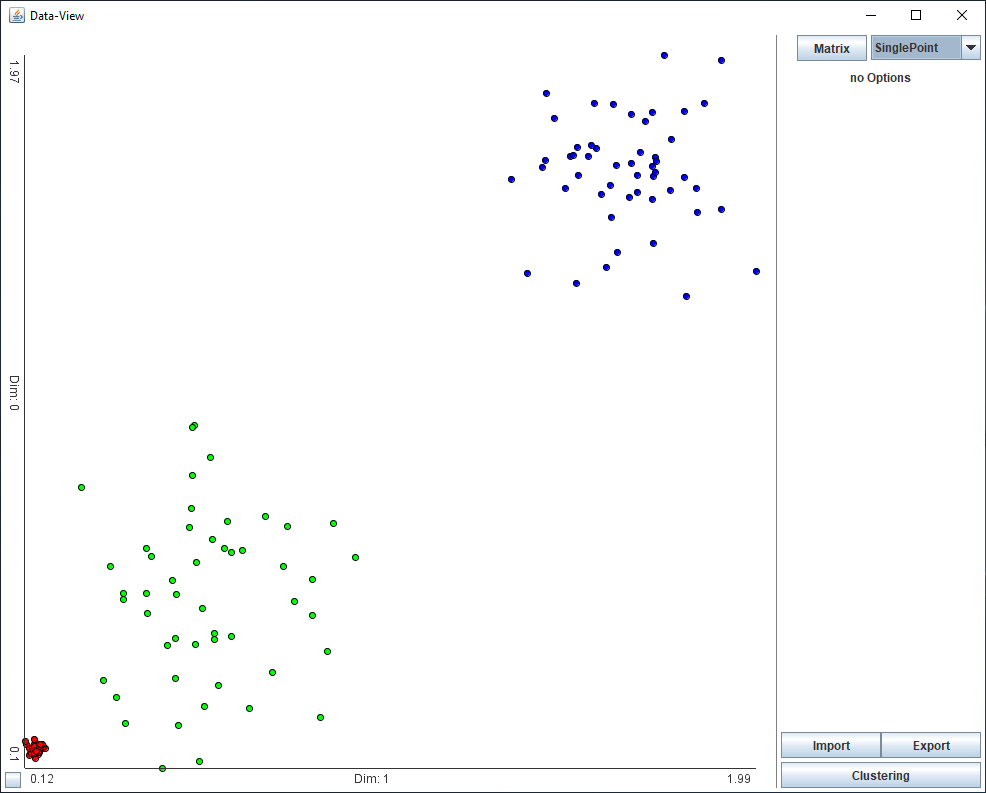
\includegraphics[scale=.4]{better_base}
	\caption{Synthetic Data with Ground Truth}
	\label{fig:better_base}
\end{figure}
\begin{figure}[h]
	\centering
	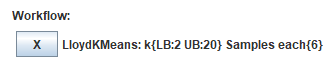
\includegraphics[scale=.75]{better_base_wf}
	\caption{Workflow for example Data-Set in Figure \ref{fig:better_base}}
	\label{fig:better_base_wf}
\end{figure}
\begin{figure}[h]
	\centering
	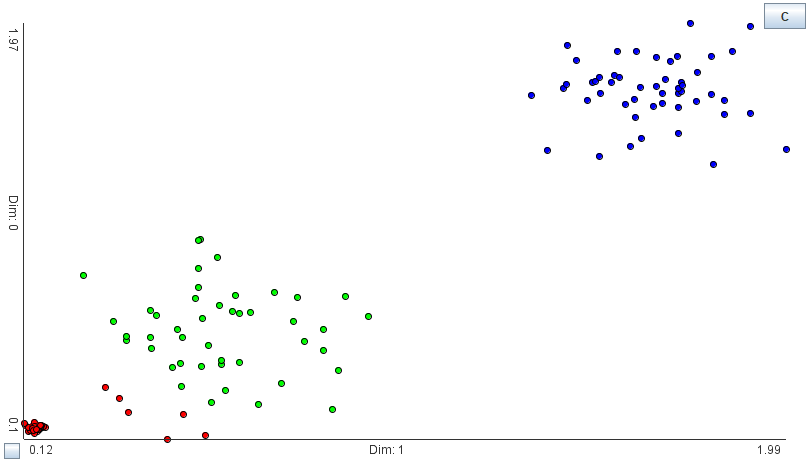
\includegraphics[scale=.4]{better_base_best}
	\caption{Result of best k-Means run for example Data-Set in Figure \ref{fig:better_base}}
	\label{fig:better_base_best}
\end{figure}
\begin{figure}[h]
	\centering
	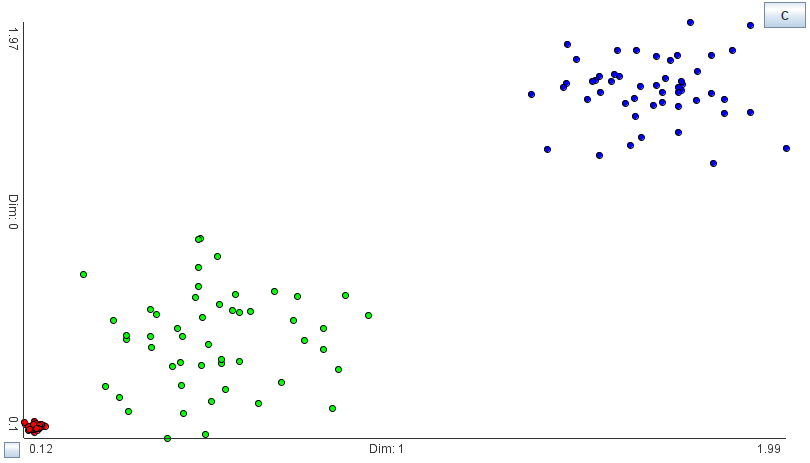
\includegraphics[scale=.4]{better_base_consensus}
	\caption{Consensus Result for example Data-Set in Figure \ref{fig:better_base}}
	\label{fig:better_base_consensus}
\end{figure}

To illustrate this, a synthetic data-set with three Gaussian distributed clusters with different standard deviations is used in this example, it can be seen in Figure \ref{fig:better_base}.

Now as this data-set is quite simple, let us create the base clusterings using Lloyd's k-Means algorithm. To increase the knowledge that can be extracted from the results, $k$ can simply be sampled in a large range. In this example, it is sampled in the range of $2$ to $20$ computing $6$ results for each $k$, see Figure \ref{fig:better_base_wf}. Using such a larger range, even if an approximate $k$ is known is often useful as the additional information of possible smaller local clusters can be integrated. Also, as a poor value for $k$ leads to less robust results, the clusterings should differ more strongly and the randomness of the result should not make the information from small clusters to dominant.

The best result resulting from a single clustering run is for k-Means with $k=3$ with a Normalized Mutual Information (NMI) score of around $0.886$. This result can be seen in Figure \ref{fig:better_base_best} 

One can see that the simple k-Means algorithm has difficulties with clusters with strongly differing spread and assigns points belonging to the green cluster to the red one. One way to fix this problem could be to use a better fitting algorithm like EM clustering, though such a choice may not be obvious with higher-dimensional data. To still find a good result, the information gathered from the other runs can be included through consensus clustering. Using the Co-Association Matrix with Average Link strategy and trusting the Lifetime criterion for the choice of $k$ we obtain exactly the same cluster assignments as in the ground truth, see Figure \ref{fig:better_base_consensus}. Here, all clusterings were included for consensus by dragging the threshold bar in the OPTICS plot to the very top.

With the information of all clusterings taken into account through consensus clustering, the consensus result has an NMI of $1$ when compared with the ground truth, showing that this combined result is better than any individual run, as it is not only similar but equal to the ground truth. Still, it is important to note that the Lifetime criterion may fail to find an ideal choice for $k$ automatically. To overcome this, DICLENS can alternatively be used as it is better at defining $k$ although it has a much higher computational cost. It is also always possible to define $k$ by hand whenever this information is available.

\subsubsection{DBSCAN}
Another data-set for which this method works is Zahn's Compound \cite{1671676} which combines multiple difficult clustering tasks. The combined data-set can be seen in \ref{fig:zahn} with its intended labels. If was standardized first, to be able to easier define DBSCAN parameters.

\begin{figure}[h]
	\centering
	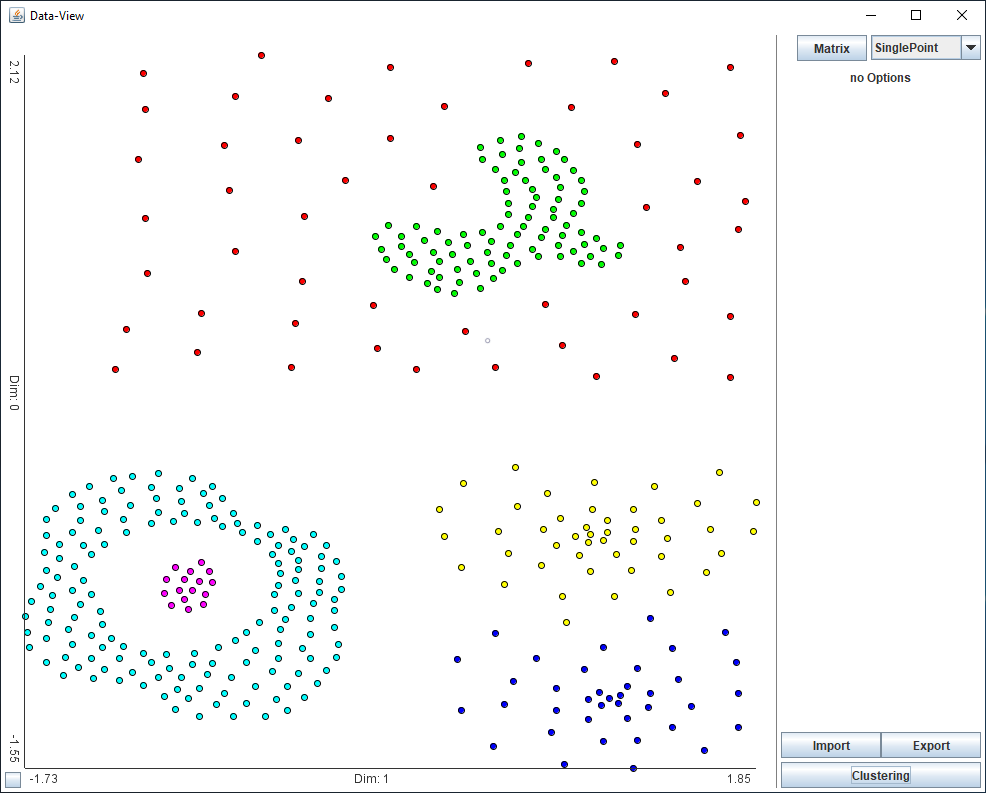
\includegraphics[scale=.4]{zahn}
	\caption{Zahn's Compound Data-Set with Labels \ref{fig:better_base}}
	\label{fig:zahn}
\end{figure}

Sampling 200 runs of DBSCAN by fixing minPTS to $5$ and randomly picking $\epsilon$ between $0.01$ and $0.5$ (which is roughly the range where non-trivial clusterings can result) gives us its best result with an NMI of $0.896$. It can be seen in Figure \ref{fig:zahn_best}. The points colored in white in Figure \ref{fig:zahn_best} indicate points that DBSCAN considered noise, for the calculation of the NMI and in all other parts of the tool they are considered to belong to a common cluster.

\begin{figure}[h]
	\centering
	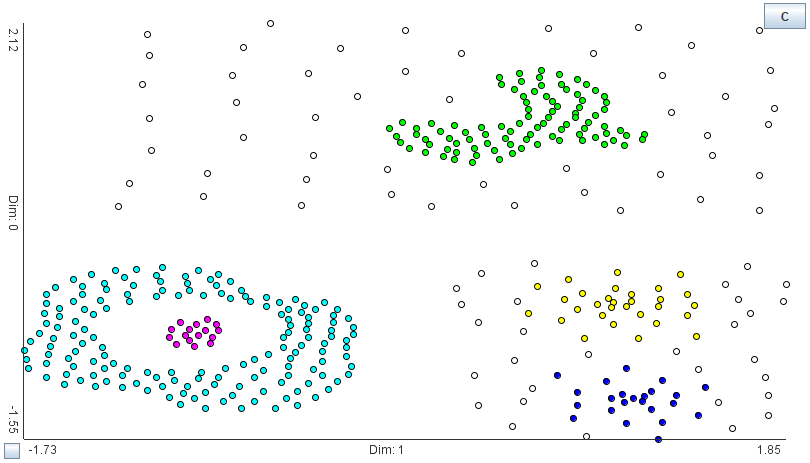
\includegraphics[scale=.4]{zahn_best}
	\caption{Best single Clustering Result for Zahn's Compound Data-Set}
	\label{fig:zahn_best}
\end{figure}
\begin{figure}[h]
	\centering
	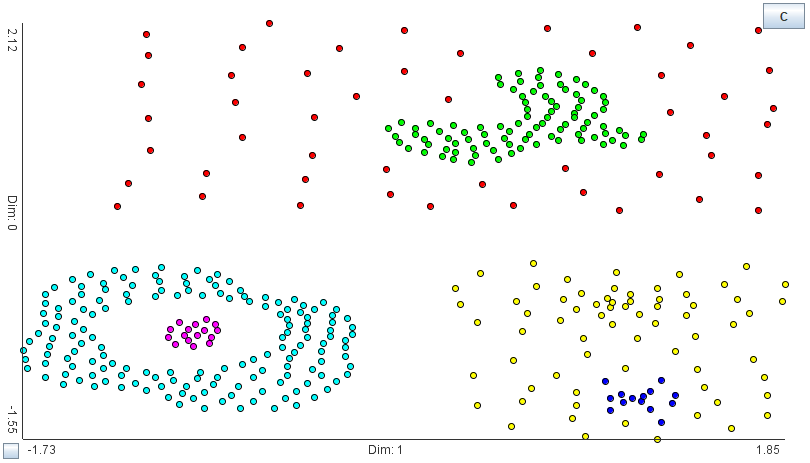
\includegraphics[scale=.4]{zahn_consensus}
	\caption{Consensus Result for Zahn's Compound Data-Set}
	\label{fig:zahn_consensus}
\end{figure}

While this result is not too bad for such a complex data-set it is not obvious to find from all of the $200$ solutions. Especially when the structure is as complex as here, it may be difficult for the user to figure out which of the results is satisfactory, given no ground truth. Consensus not only gives us a better solution (fixed $k=6$) with an NMI of $0.943$ but also only a single result. This means that besides improving the quality of the result the user does therefore not need to choose the right solution. The output of the consensus function can be seen in Figure \ref{fig:zahn_consensus}. The used consensus function was once again the  Co-Association Matrix based one.

\subsubsection{Real Data}

The same strategy as for the example data in Figure \ref{fig:better_base} was tested with the Iris data-set \cite{Dua:2019}, the first two dimensions of this data-set can be seen in the user testing section in Figure \ref{fig:iris}. Here, Lloyd's k-Means was also used and the parameter $k$ was sampled in the range between $2$ and $10$, computing $10$ samples per value $k$. The best result when compared to the ground truth was for $k=3$ with an NMI of $0.757$ while computing the consensus for all clusterings resulted in a solution with an NMI of $0.797$ (with $k=3$ for the consensus function). This shows once again the value of consensus clustering as it can eliminate the need of evaluating individual solutions with quality measures and picking one, while still finding a good or even better solution. Still, one should aim to find the method that simplest explains the data, for which consensus results are usually no good candidate. 

Besides the Iris data-set, a real wireless indoor localization data-set \cite{wireless} was used as a test-case for a user, more on this can be found in Section \ref{sec:user_test}. There can be seen that the parameter $k$ can be found as a side-effect of collecting consensus solutions for meta-clusters and better results than the individual runs can be obtained. This effect of obtaining $k$ can also further be observed in the example in Section \ref{sec:multi_sol}.

\section{Unobtainable Solutions}\label{sec:unob}
Single clustering algorithms may not be able to find the structure of a data-set when multiple different kinds of structures are present for individual clusters. Combining results of different clustering algorithms may solve this problem, as correctly identified structures should be robust throughout multiple runs of a fitting algorithm while they should not be robust whenever the algorithm doesn't fit the structure. To illustrate this a data-set was created combining a U-shaped density based cluster with Gaussian clusters with different deviations, see Figure \ref{fig:unob}.

\begin{figure}[h]
	\centering
	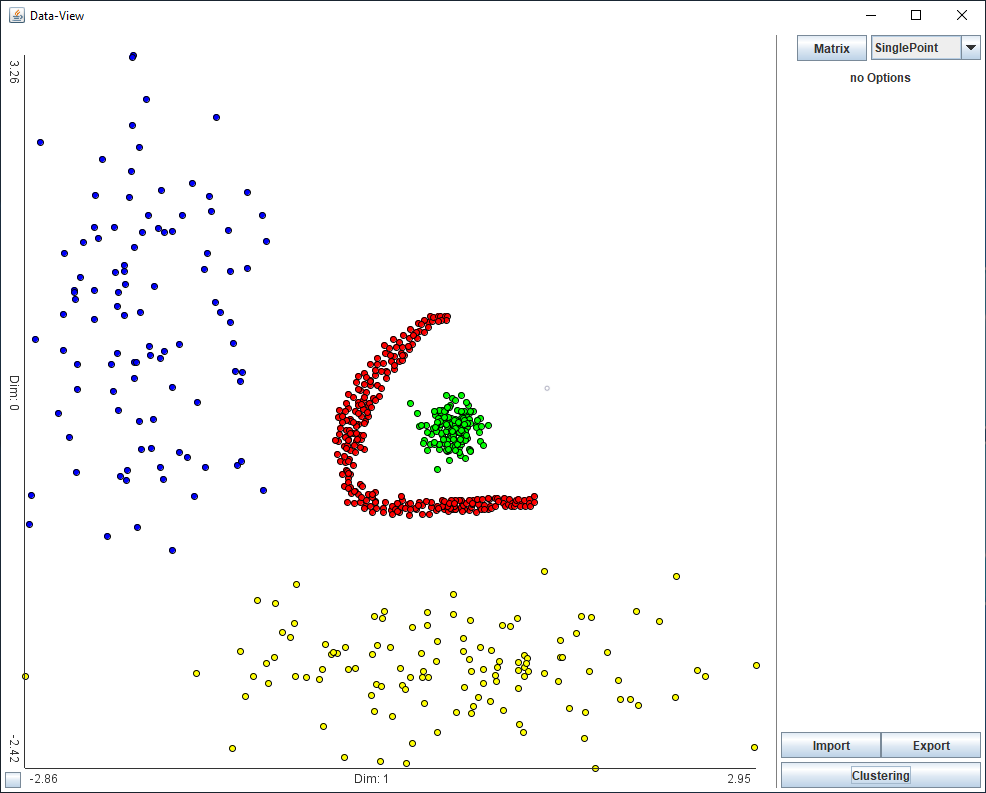
\includegraphics[scale=.4]{unob}
	\caption{Example Data-Set with different Cluster-Structures and Labels}
	\label{fig:unob}
\end{figure}

To produce base clusterings k-Means was run choosing $k$ between $2$ and $20$ creating $5$ results each and DBSCAN was run with $minPTS=5$ and $\epsilon$ between $0.01$ and $0.5$ taking $100$ samples. The seed was again fixed at $1$  for reproducibility and trivial solutions were omitted. Also, these ranges were selected such that a large diversity of solutions is obtained while not creating trivial clusterings. Trivial clusterings are not desired in this process as all points either being in one or each point in an individual cluster is no useful information. The workflow can be seen in Figure \ref{fig:unob_wf}.

\begin{figure}[h]
	\centering
	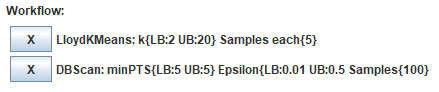
\includegraphics[scale=.75]{unob_wf}
	\caption{Workflow for example Data-Set in Figure \ref{fig:unob}}
	\label{fig:unob_wf}
\end{figure}

\begin{figure}[h]
	\centering
	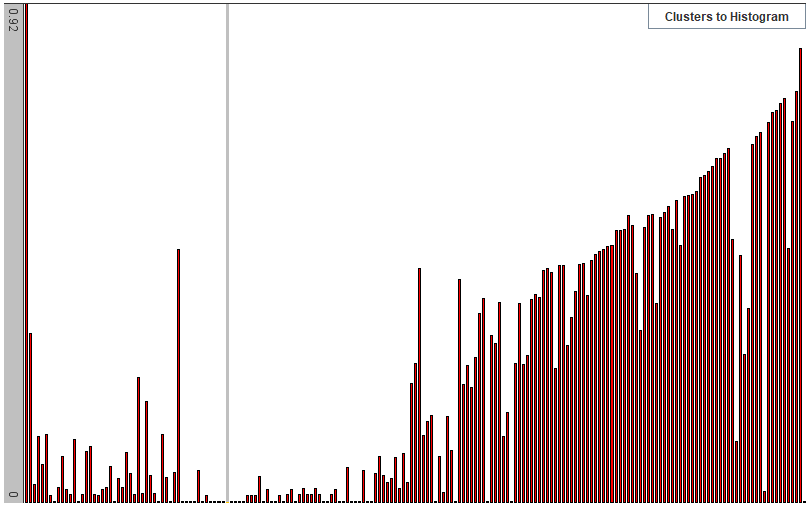
\includegraphics[scale=.4]{unob_optics_stable}
	\caption{OPTICS reachability plot for Workflow in Figure \ref{fig:unob_wf}}
	\label{fig:unob_optics_stable}
\end{figure}

When looking at the OPTICS reachability plot, one can see that a dense region of clustering results can be found, see Figure \ref{fig:unob_optics_stable}. Results that occur in this region can be regarded as robust and should represent a good result, but in this example no algorithm can find the true structure of the data. For example, the clustering selected in Figure \ref{fig:unob_optics_stable} can be deemed robust and also visually seems sensible, but it does not capture the nature of the data, as can be seen in Figure \ref{fig:unob_stable}. As the reachability plot also shows multiple valleys, a fair conclusion could be that different equally valid solutions exist. Still, for this clustering problem, we know that the structure cannot be found with a single algorithm and one can assume that the robust regions only represent good results for different parts of the data. 

Looking at the results of the different algorithms exactly this behavior can be observed, see Figure \ref{fig:single}.

\begin{figure}[h]
\centering
\begin{subfigure}[t]{.49\textwidth}
  \centering
  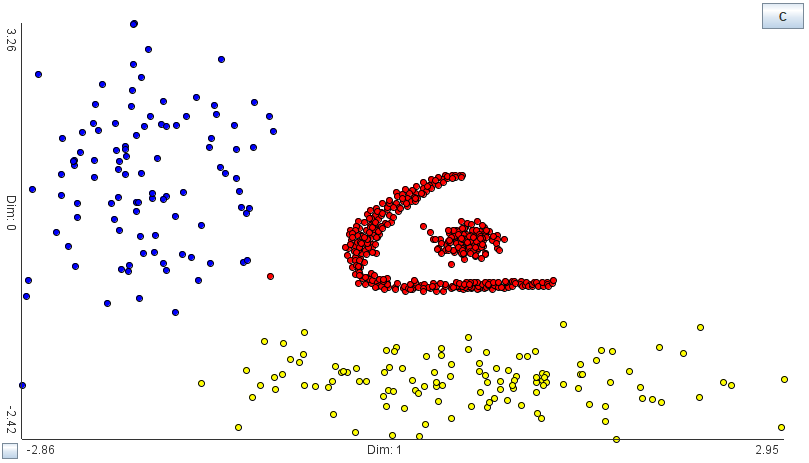
\includegraphics[width=.95\linewidth]{unob_k3}
  \caption{K-Means with $k=3$}
  \label{fig:unob_k3}
\end{subfigure}
\hfill
\begin{subfigure}[t]{.49\textwidth}
  \centering
  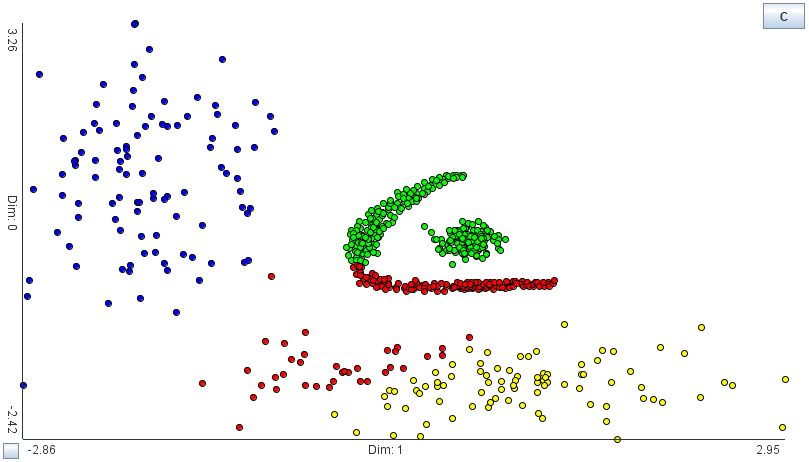
\includegraphics[width=.95\linewidth]{unob_k4ex}
  \caption{K-Means with $k=4$}
  \label{fig:unob_k4ex}
\end{subfigure}
\medskip
\begin{subfigure}[t]{.49\textwidth}
  \centering
  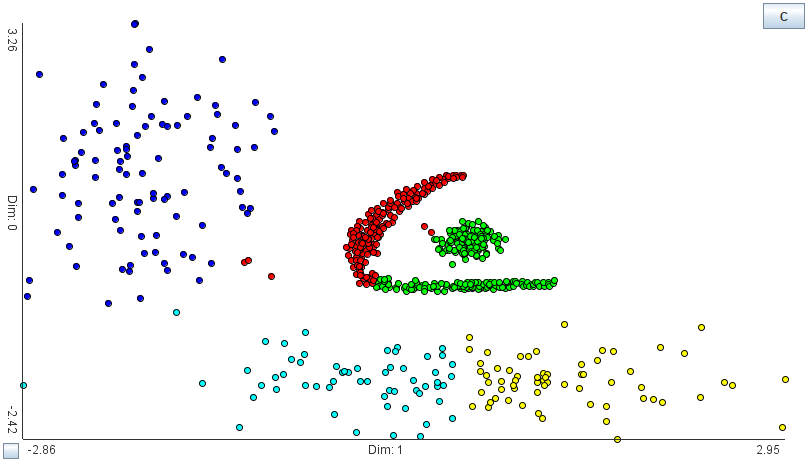
\includegraphics[width=.95\linewidth]{unob_k5ex}
  \caption{K-Means with $k=5$}
  \label{fig:unob_k5ex}
\end{subfigure}
\hfill
\begin{subfigure}[t]{.49\textwidth}
  \centering
  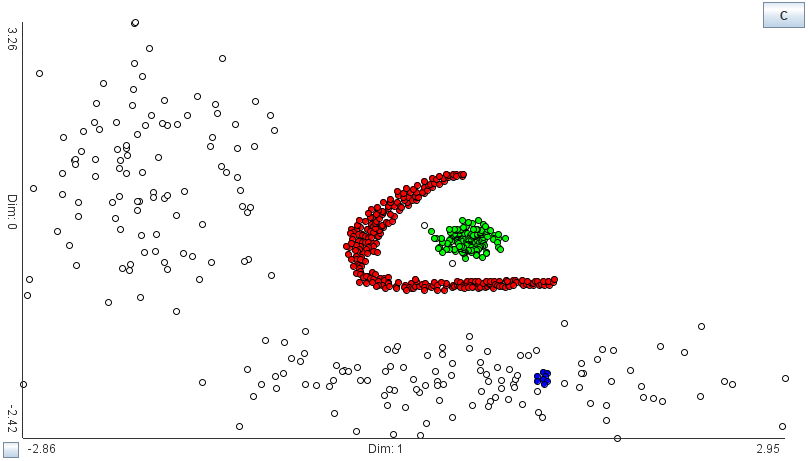
\includegraphics[width=.95\linewidth]{unob_best}
  \caption{DBSCAN, the best single Clustering Result}
  \label{fig:unob_best}
\end{subfigure}
\medskip
\begin{subfigure}[t]{.49\textwidth}
	\centering
	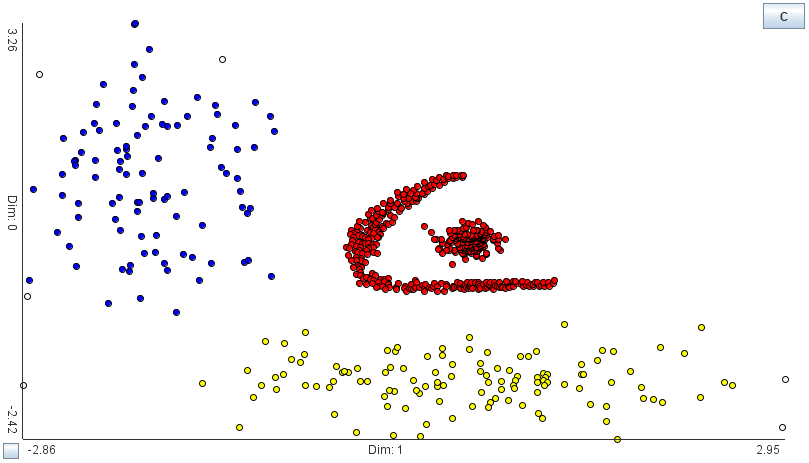
\includegraphics[width=.95\linewidth]{unob_stable}
	\caption{Selected robust Clustering from Figure \ref{fig:unob_optics_stable}}
	\label{fig:unob_stable}
\end{subfigure}
\caption{Single Clustering results for Data-Set in Figure \ref{fig:unob}}
\label{fig:single}
\end{figure}


Here, the red cluster can not be found with partitioning methods such as k-Means and either the green or the blue and yellow clusters can not be found by density-based methods. Both the k-Means result for $k=3$ (Figure \ref{fig:unob_k3}) and some DBSCAN results (Figure \ref{fig:unob_best}) can be found in valleys of the reachability plot but none of both is able to find the structure of all clusters.

\begin{figure}[h]
	\centering
	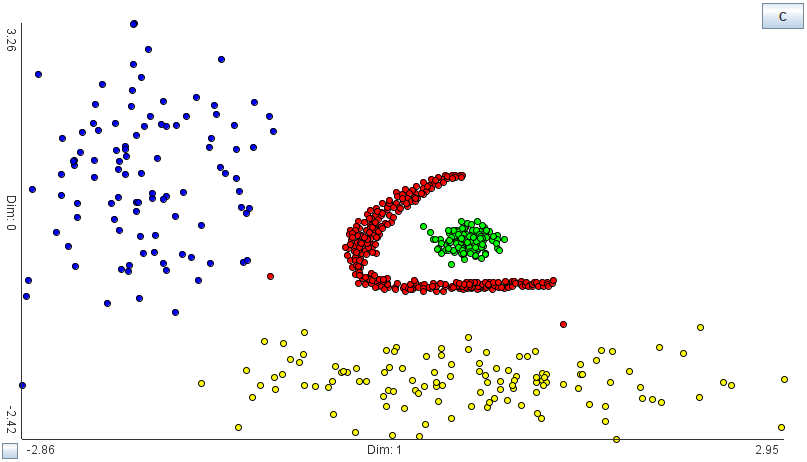
\includegraphics[scale=.4]{unob_consensus}
	\caption{Consensus Result for Data-Set in Figure \ref{fig:unob}}
	\label{fig:unob_consensus}
\end{figure}

To solve this consensus clustering can be performed. As discussed previously both kinds of results have produced robust clusterings and the most relevant information can be combined into a better common result. In this example DICLENS was selected, fixing $k=4$ and the final result was computed. As can be seen in Figure \ref{fig:unob_consensus}, using the information available from all solutions, both the k-Means and DBSCAN runs, finds a result very close to the ground truth. This result has only a few misclassified points, most noticeably the two red points outside the U-shaped cluster. The NMI of the consensus result is $0.978$ while the best result of a single run (Figure \ref{fig:unob_best}) has an NMI of $0.872$. This large improvement shows the power of using consensus clustering when different structures are present in the data.


\section{Multiple Solutions}\label{sec:multi_sol}
Finding which clustering solution is best for an unexplored data-set can be non-trivial. Other visual frameworks often use quality metrics, which may be biased towards specific structures. In this section, I want to present you with this problem using the newly created tool and show that robustness can be used to find good results. For this, the unlabeled data-set shown in Figure \ref{fig:multi} is used as an example.

\begin{figure}[h]
	\centering
	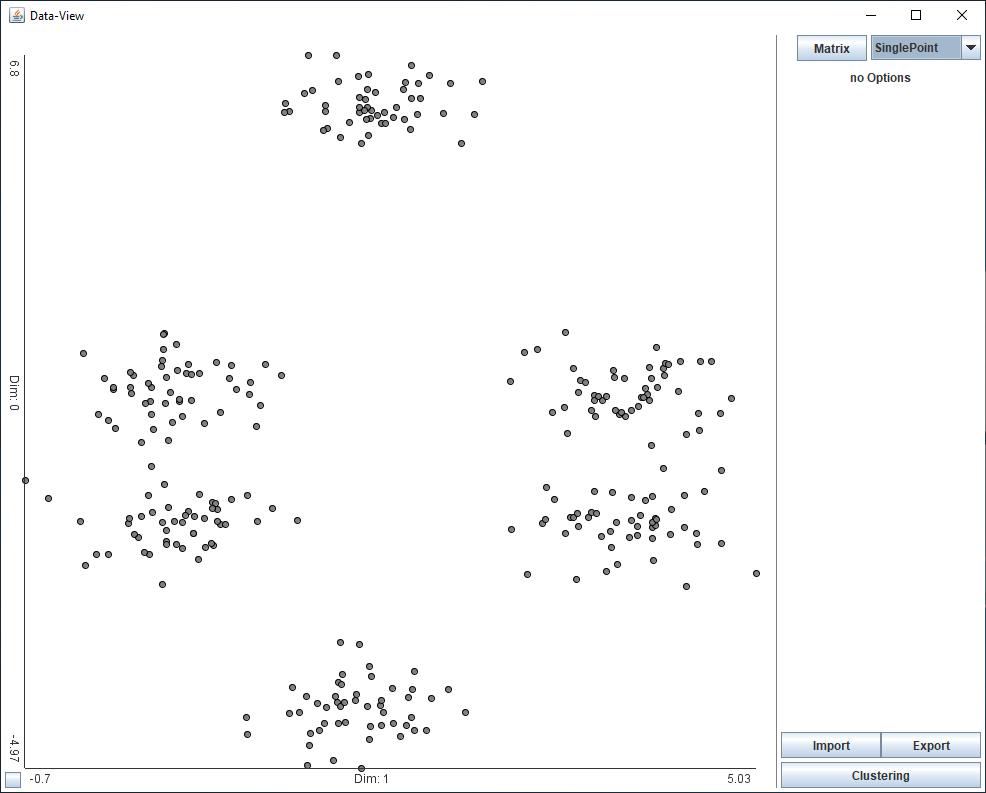
\includegraphics[scale=.4]{multi}
	\caption{Example Data-Set with unknown Labels}
	\label{fig:multi}
\end{figure}

Visually, it is already difficult to decide how many clusters can be seen. The points on the left and right can be seen as one or two clusters each, but one could even claim that one side consists of one and the other two clusters. For this, small data-set such claims can still easily be made but with more dimensions, such thoughts become more complex. For this reason, I will show how different results can be found using this tool, by regarding indicators of robustness for the results.

To generate base clusterings k-Means was used, varying the value for $k$ between $2$ and $10$ and computing $10$ samples for each value. Trivial solutions were omitted and no ground truth was added as none is available. With the workflow defined, it is executed also performing OPTICS for meta-clustering using the default MinPTS and $\epsilon$. With the ordering resulting from the OPTICS algorithm, the heat map for the resulting clusterings is created and can be seen in Figure \ref{fig:multi_heatmap}.

\begin{figure}[h]
	\centering
	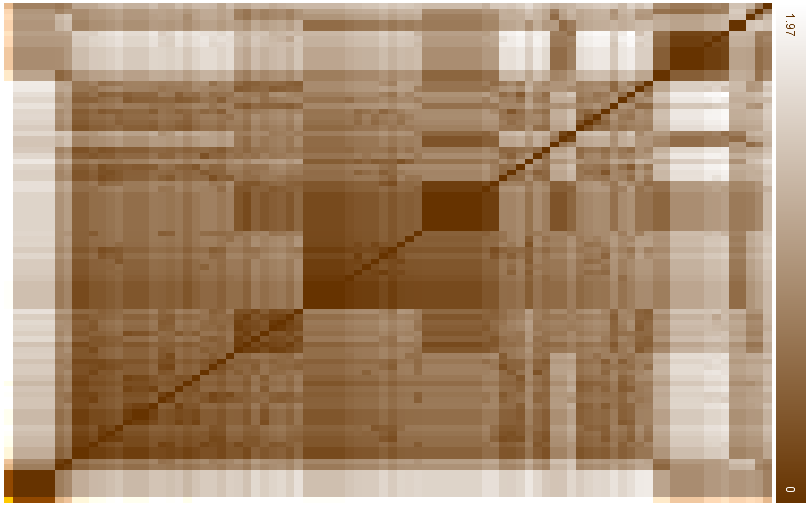
\includegraphics[scale=.4]{multi_heatmap}
	\caption{Heat Map of Meta-Clustering for Data-Set in Figure \ref{fig:multi}}
	\label{fig:multi_heatmap}
\end{figure}

In this heat map, hierarchical structures of similar clustering results can already be observed. Darker rectangles near the diagonal show regions with similar clustering results, indicating their robustness as many different runs found similar results. This meta-cluster structure can more clearly be defined in the OPTICS reachability plot, as seen in Figure \ref{fig:multi_optics}, whereby the threshold is set such that valleys are separated and noise is left out. With this, the meta-clusters are defined each representing a group of similar and therefore hopefully robust clustering solutions.

\begin{figure}[h]
	\centering
	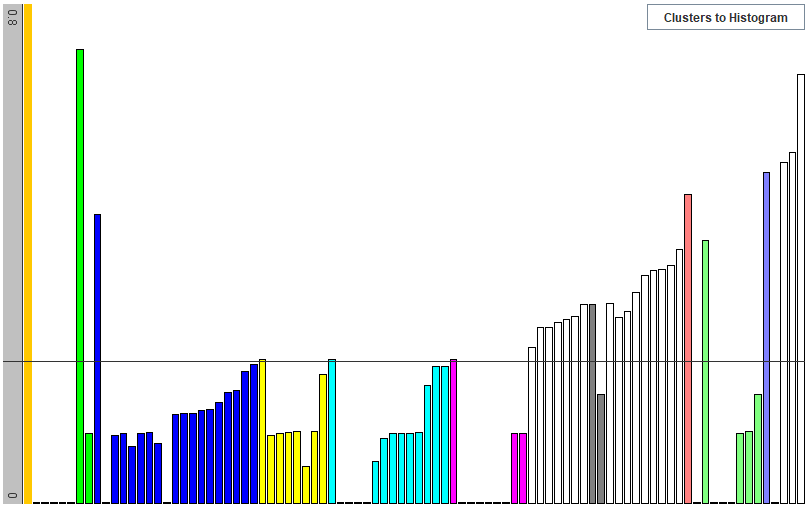
\includegraphics[scale=.4]{multi_optics}
	\caption{OPTICS Plot of Meta-Clustering for Data-Set in Figure \ref{fig:multi}}
	\label{fig:multi_optics}
\end{figure}

To create result candidates, the consensus is computed with the Co-Association Matrix algorithm with Average Link strategy (Lifetime criterion) and letting the function guess $k$ by itself. This way, as many consensus results are obtained as meta-clusters are available, each one representing the merged knowledge of its meta-cluster. The most interesting results should then be the ones that included many base clusterings, i.e. where the meta-cluster was large. This should be a fair assumption as the definition of the threshold fixes how similar clusterings need to be to be deemed robust and meta-clusters with many solutions should therefore be especially robust. For this reason, the number of merged base clusterings can be used as an implicit ranking of the consensus solutions. Figure \ref{fig:multi_consres} shows the consensus results for the four largest meta-clusters with the corresponding number of included base clusterings.

\begin{figure}[h]
\centering
\begin{subfigure}[t]{.49\textwidth}
  \centering
  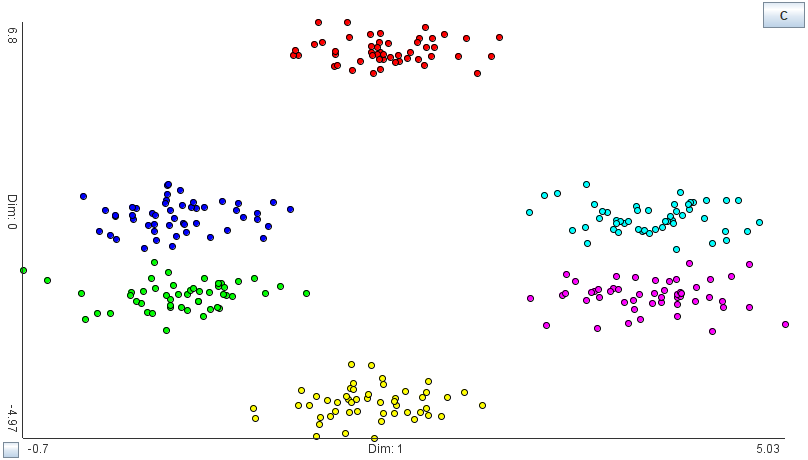
\includegraphics[width=.95\linewidth]{multi_c6}
  \caption{Consensus Result for blue Cluster\\(19 base clu.)}
  \label{fig:multi_c6}
\end{subfigure}
\hfill
\begin{subfigure}[t]{.49\textwidth}
  \centering
  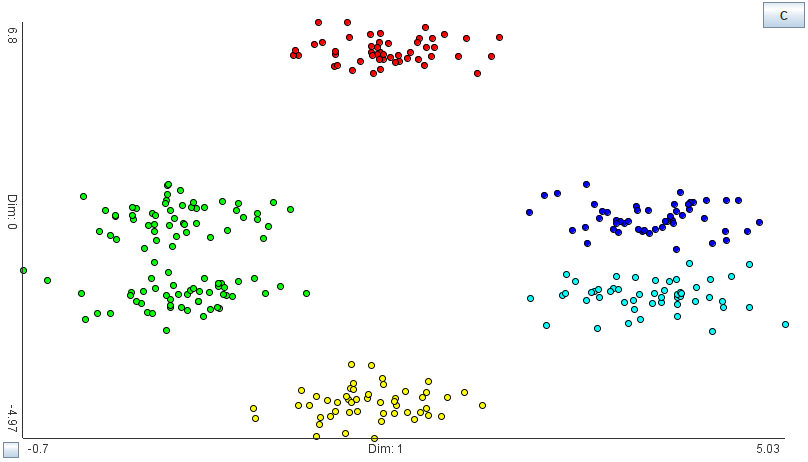
\includegraphics[width=.95\linewidth]{multi_c5_2}
  \caption{Consensus Result for light-blue Cluster (14 base clu.)}
  \label{fig:multi_c5_2}
\end{subfigure}
\medskip
\begin{subfigure}[t]{.49\textwidth}
  \centering
  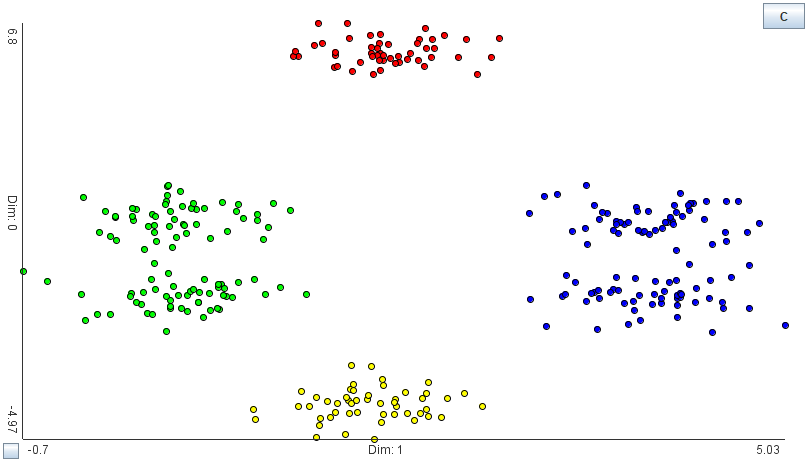
\includegraphics[width=.95\linewidth]{multi_c4}
  \caption{Consensus Result for pink Cluster\\(9 base clu.)}
  \label{fig:multi_c4}
\end{subfigure}
\hfill
\begin{subfigure}[t]{.49\textwidth}
  \centering
  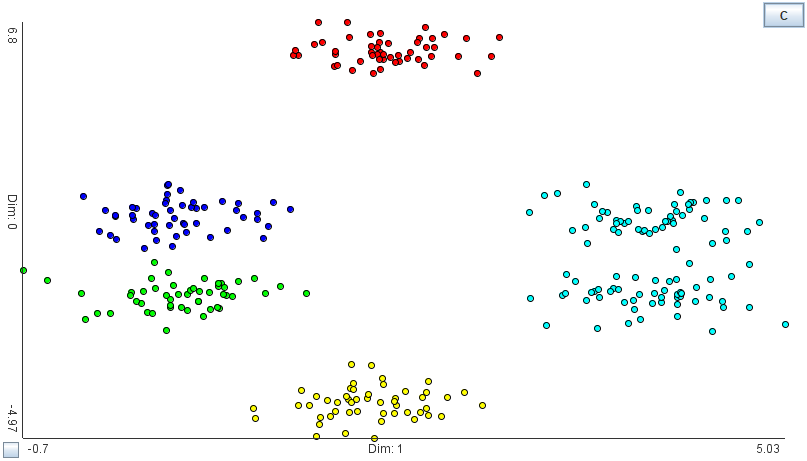
\includegraphics[width=.95\linewidth]{multi_c5_1}
  \caption{Consensus Result for yellow Cluster\\(8 base clu.)}
  \label{fig:multi_c5_1}
\end{subfigure}

\caption{Consensus Clustering results for Data-Set in Figure \ref{fig:multi}}
\label{fig:multi_consres}
\end{figure}

Analyzing those results, one can see that the intuition mentioned before was also found by the consensus results for the largest meta-clusters. The largest meta-cluster, which included 19 base clusterings, resulted in a consensus clustering whereby $6$ clusters were found (see Figure \ref{fig:multi_c6}). This result can be seen as the highest-ranked one and therefore most robust as it includes the largest number of clusterings deemed robust. The second and fourth largest meta-clusters found that the left or right group should be in a common cluster respectively (Figure \ref{fig:multi_c5_2} and \ref{fig:multi_c5_1}) while the third-largest one considers both of them as one large cluster each (Figure \ref{fig:multi_c4}). The robustness of the result with $6$ clusters can also further be seen when the consensus overall base clusterings is computed. Even without setting a parameter $k$ for this computation the result is equivalent to the one in Figure \ref{fig:multi_c6}.

Finding more than one possible result can be helpful on top of only creating one final one, as knowledge may be gained. In this simple case, it is easy to recognize how the left and right groups of points relate to each other but for more complex data-sets this may difficult to see. Here, it would for example be beneficial to look at what the underlying reason for the layout of the points may be, such that one can properly reason why a group of points should be one or two clusters. Also, note that in no part of this process quality metrics are needed, only the definition of the meta-cluster through the threshold should be done in a sensible way. In general, a good choice for this should be to visually analyze which cut-off value creates visually pleasing valleys, as well as considering how fine-grained one wants the differences between the results to be.

This way of finding multiple solutions may also prove useful when a data-set may be clustered with different goals. For example, clustering patient data could be done to find groups of patients with different kinds of cancer or different kinds of diabetes. Even though both may cluster on the same data-set (for example vectorized patient data), the desired clusterings are likely to differ and different algorithms and parameter-sets may reflect this.

\section{User Testing}\label{sec:user_test}
To experimentally test how easy it is to find good clustering solutions three test-scenarios where created and a fellow computer science student was tasked to find solutions and explain his findings. To again make the results reproducible the random seed was fixed at $1$ and the ground truth was not shown to the user.

The first data-set (QCM3) \cite{qcm} includes QCM sensor data where different types of alcohol were passed through the sensor in different concentrations. The task was to find how many types of alcohol were tested and to find the clusters representing each type.
%%img?

At first, the user tried sampling k-Means with $k$ in the range $2$ to $20$ creating $10$ solutions each. Doing this, he looked at which values for $k$ resulted in outlying/non-robust results. When filtering for solutions with $\leq10$ clusters, it was easy to see that the results with more than $10$ clusters produce poor solutions. The effect of which clusterings are filtered out this way can be seen in Figure \ref{fig:user_qcm_optics}.

\begin{figure}[h]
	\centering
	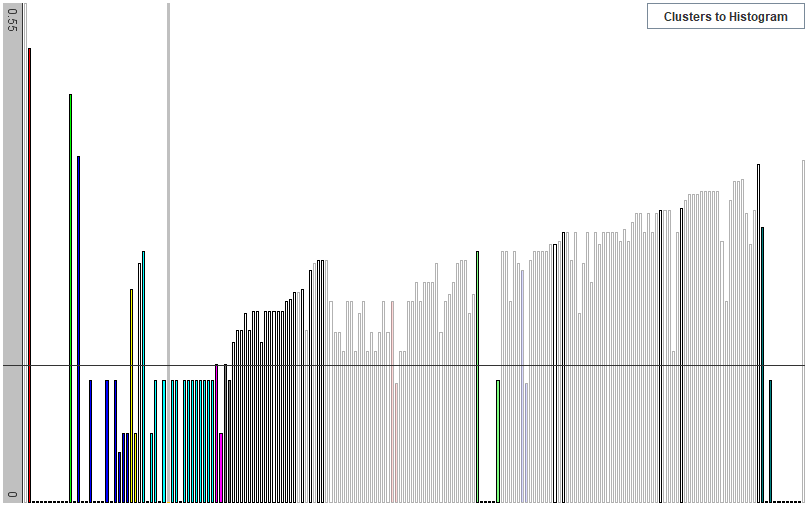
\includegraphics[scale=.5]{user_qcm_optics}
	\caption{OPTICS Plot with applied Filter}
	\label{fig:user_qcm_optics}
\end{figure}

With this knowledge, the clusterings were re-computed only using $k$ in the range $2$ to $10$. The resulting reachability plot now more clearly shows robust groups of solutions, the threshold choice of the user can be seen in Figure \ref{fig:user_qcm_optics2}.

\begin{figure}[h]
	\centering
	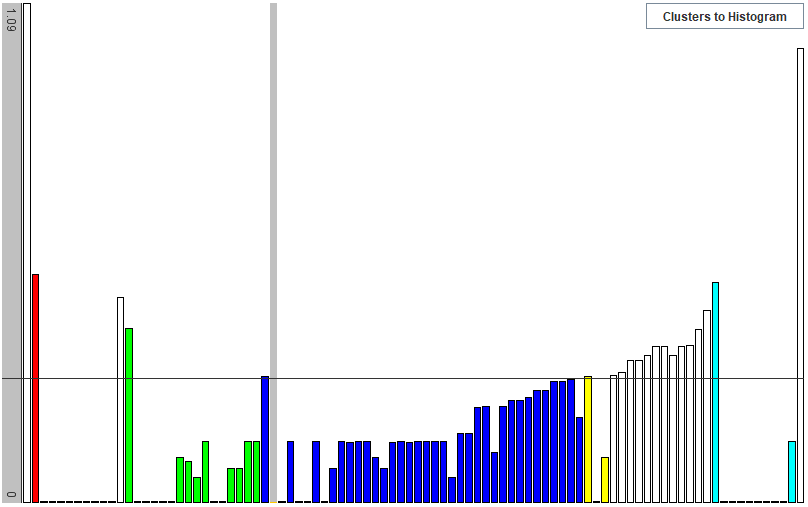
\includegraphics[scale=.5]{user_qcm_optics2}
	\caption{OPTICS Plot after improved Sampling}
	\label{fig:user_qcm_optics2}
\end{figure}

For deciding on the final solution, he applied the default consensus function and obtained 5 results, one for each meta-cluster. From these solutions, he chose the one resulting from the largest meta-cluster, with the reasoning that the threshold definition found it to be the largest group of robust solutions. The chosen result included 5 clusters which the user claimed to be the number of types of alcohol in the data-set. Not only is this the right number of clusters, but the obtained result is also $100\% $ equivalent to the ground truth. He also observed that the next largest meta-cluster produced a result where two clusters were merged into one. When visually inspecting the first and second result it also seems that this merging could be a sensible choice.

The second data-set \cite{wireless} contains signal strength data from smartphones where the strength of seven nearby wireless networks is collected for each smartphone. The task is to find how many smartphones are in the area of these wireless networks and assign the measurements taken to the smartphones. The first two dimensions (wifi access-points) can be seen in Figure \ref{fig:user_wifi_gt}, the coloring is according to the ground truth.

\begin{figure}[h]
	\centering
	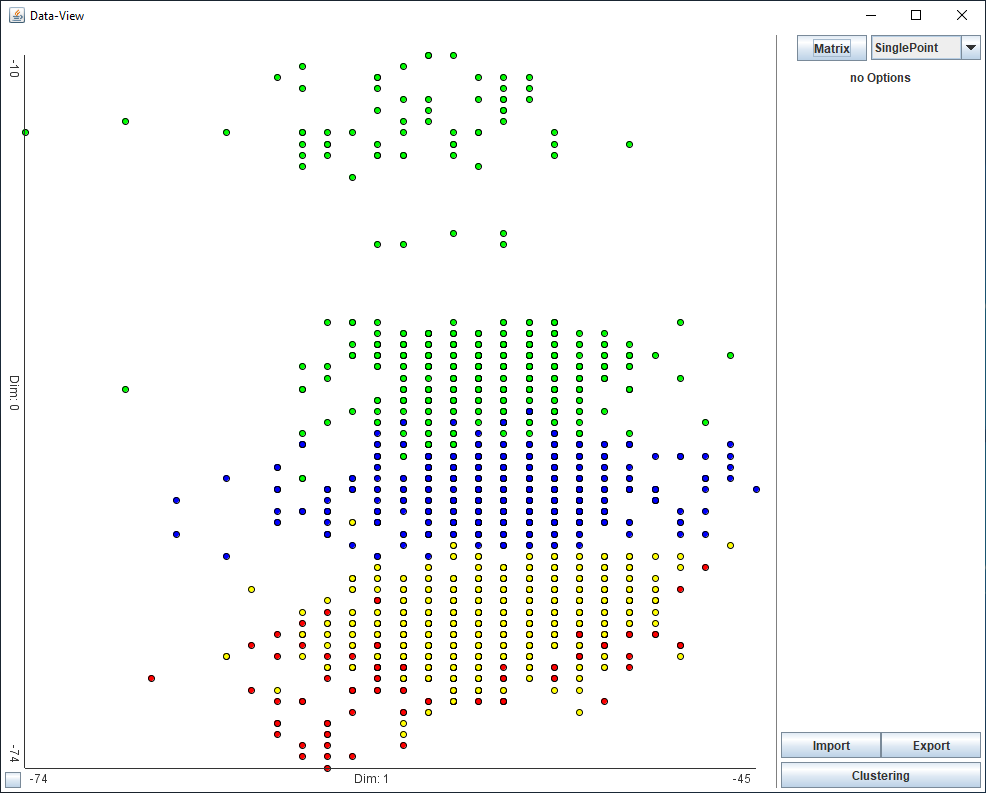
\includegraphics[scale=.4]{user_wifi_gt}
	\caption{WiFi Localization Data-Set with first two Dimensions shown}
	\label{fig:user_wifi_gt}
\end{figure}

To start off, the user tried creating clustering solutions using DBSCAN, but in both the reachability plot and the heat map it could be seen that no robust solutions except nearly trivial ones could be found. In most cases, the points were either nearly all assigned to one cluster or different small clusters each. With this information, he deducted that the algorithm is probably not fit for finding a good solution and chose to use k-Means. There, as he did not know how many clusters are in the data-set, he sampled $k$ from $2$ to $50$ and found again that solutions with $k>20$ seemed poor. He decided on this value, just like in the first example, by finding where solutions begin to differ strongly. The resulting reachability plot is shown in Figure \ref{fig:user_wifi_optics}

\begin{figure}[h]
	\centering
	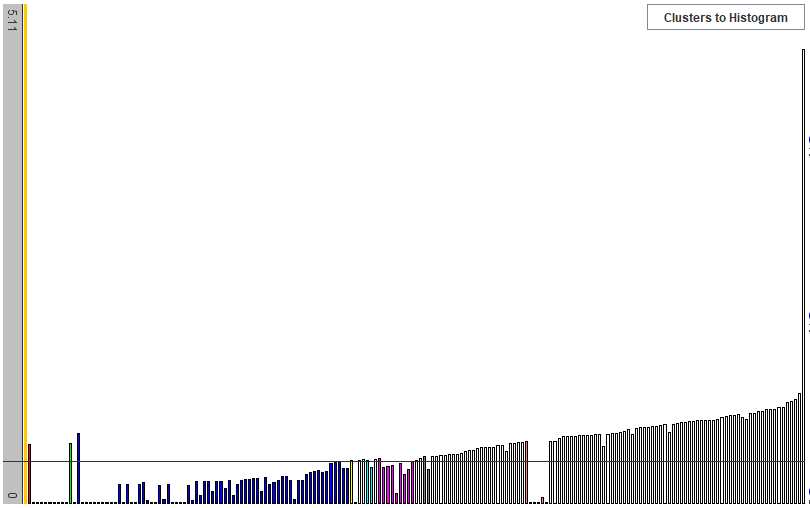
\includegraphics[scale=.5]{user_wifi_optics}
	\caption{OPTICS Plot for WiFi Localization Data-Set}
	\label{fig:user_wifi_optics}
\end{figure}

With the defined meta-clusters, the user used the consensus calculation to obtain the solutions from each meta-cluster. From those, he again chose the result which included the largest number of clusterings in the meta-cluster. This solution can be seen in Figure \ref{fig:user_wifi_consensus}. Again, his reasoning was that as the meta-cluster is largest, the largest number of robust solutions was found in this cluster and therefore most likely combined into the best solution. When looking at the NMI of the found result, the observed value of $0.9142$ is not only very good, it is even higher than the NMI score of the best single clustering run (NMI=$0.8904$). This best simple result can be seen in Figure \ref{fig:user_wifi_best}. Note that the colors of these results are not adapted to best fit the ground truth as it was not available for the user.

\begin{figure}[h]
\centering
\begin{subfigure}[t]{.49\textwidth}
  \centering
  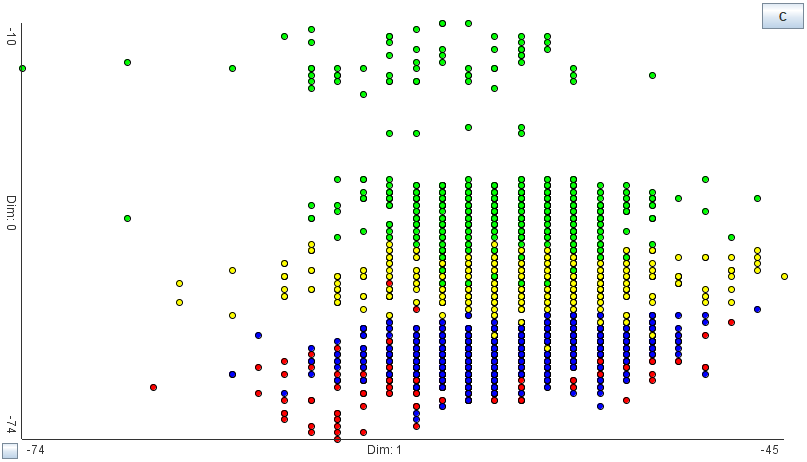
\includegraphics[width=.95\linewidth]{user_wifi_consensus}
  \caption{Consensus Result for blue (largest) Meta-Cluster}
  \label{fig:user_wifi_consensus}
\end{subfigure}
\hfill
\begin{subfigure}[t]{.49\textwidth}
  \centering
  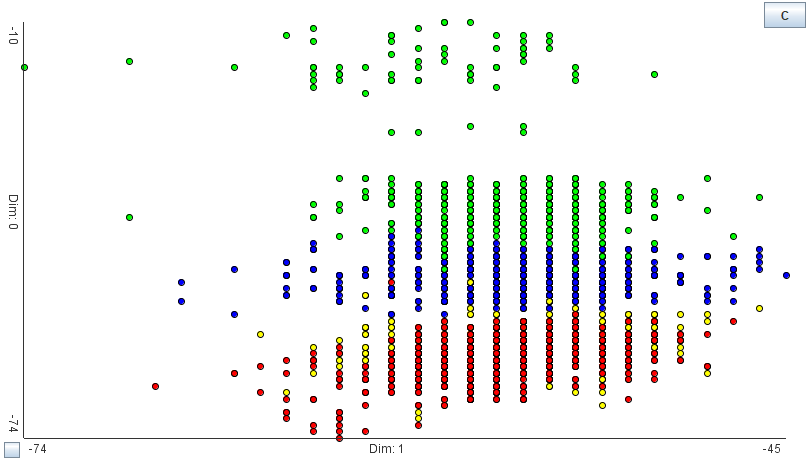
\includegraphics[width=.95\linewidth]{user_wifi_best}
  \caption{Best Result of single Clustering Run}
  \label{fig:user_wifi_best}
\end{subfigure}

\caption{Clustering results for WiFi Localization Data-Set}
\label{fig:user_wifi}
\end{figure}

These findings once again show that with little knowledge on the data one is able to find very good clustering solutions and even get an accurate estimate for the number of clusters.

Lastly, the user was tasked to find the best clustering result he can for the iris data-set \cite{Dua:2019}. For this, he was told that the set consists of three different types of flowers. The attributes collected in this set include the sepal width and length as well as the petal width an length. The first two dimensions are shown in Figure \ref{fig:iris}, there the labels represent the ground truth.

\begin{figure}[h]
	\centering
	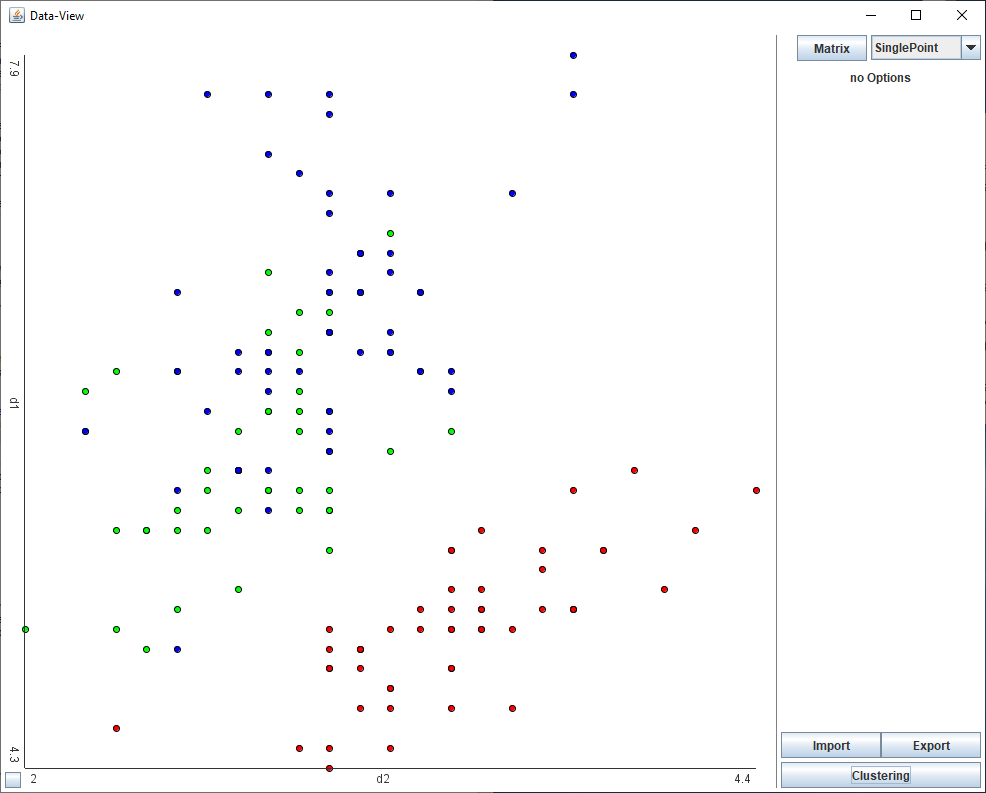
\includegraphics[scale=.4]{iris2}
	\caption{First two dimensions of Iris Data-Set}
	\label{fig:iris}
\end{figure}

The user assumed that those attributes may be Gaussian distributed with possibly different distributions and therefore chose the EM clustering algorithm. He sampled the range of $2$ to $5$ for $k$ and calculated $10$ results for each value, to also analyze solutions for different choices of $k$. Next, he changed the threshold in the reachability plot in the resulting meta-view such that visually pleasing solution groups can be seen. This choice is visualized in Figure \ref{fig:user_iris_optics}.

\begin{figure}[h]
	\centering
	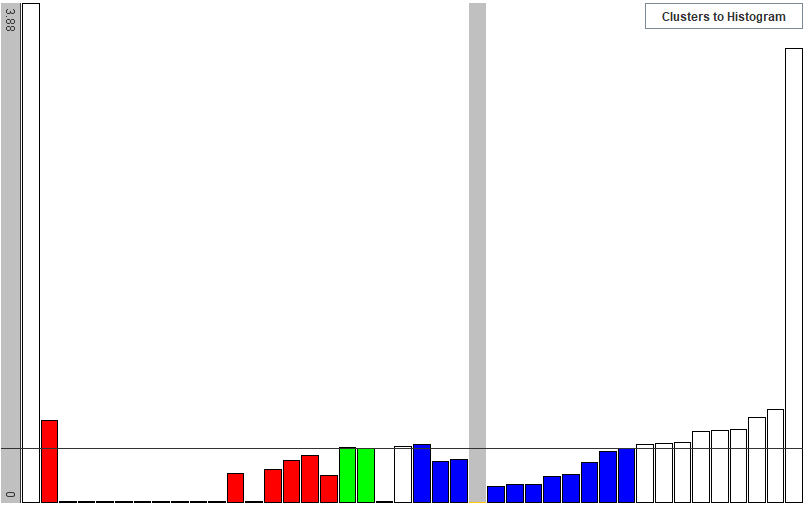
\includegraphics[scale=.4]{user_iris_optics}
	\caption{OPTICS Plot with user-defined Threshold}
	\label{fig:user_iris_optics}
\end{figure}

With this definition, he computed consensus results for all groups, which resulted in 3 solutions. As he was told that there are 3 types of flowers the consensus result for the blue meta-cluster was his choice for the final answer, which was also the best overall result. Still, he noted that without this knowledge the choice of two clusters would have been more intuitive for him as the meta-cluster included more results and seemed more robust. The NMI score of his chosen solution was $0.8997$ and this clustering solution is exactly the same as the best single clustering run, this best solution is selected in Figure \ref{fig:user_iris_optics} and shown in Figure \ref{fig:user_iris_best}. Again note that this solution is the same as the one obtained by the consensus function when selecting the result with $3$ clusters.

\begin{figure}[h]
	\centering
	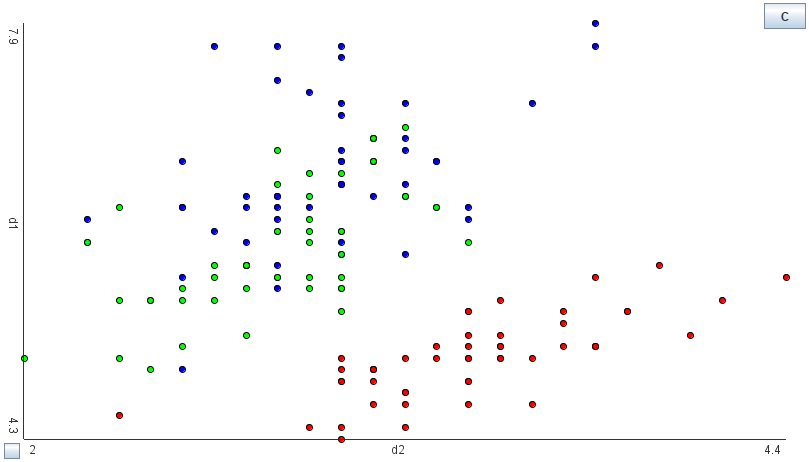
\includegraphics[scale=.4]{user_iris_best}
	\caption{First two dimensions of Clustering Solution for Iris Data-Set}
	\label{fig:user_iris_best}
\end{figure}

This shows that using the consensus function may not result in a better solution than can be found by individual clustering algorithm runs, but at least facilitates choosing the correct one out of them. Even though this solution was available, others were present, which would have been a less good choice.

\part{Concluding Thoughts}

\chapter{Future Work}\label{cha:futurework}

\section{Improvements for the Tool}
Even though the created tool already proves useful for finding good clustering solutions, further work should still be done such that it becomes more generally usable. 

A downside of the current implementation is that the focus of it lies solely on finding the best clustering result. This brings the problem that the methods implemented may not be fast enough when using a large data-set. To improve on this, the next steps should be to further optimize the methods for parallel environments and possibly implement similarly accurate but overall faster methods. This is especially true for the consensus functions as they can be very costly depending on the number of clusters in the individual results, target cluster number, number of points and dimensions in the data. Different functions runtimes depend on different subsets of these values and also vary in their accuracy. Here, more work should be put into finding the generally most accurate and performant method.

Additionally, more feedback should be given to the user on the progress of the consensus calculation. As those methods are quite complicated, the current tool does not include a progress bar for the consensus calculation, even though this may be needed as those functions may take a long time for computation. The user that worked on the examples in the previous sections also mentioned that some views are too small when many clustering runs are performed. He noted that it would be useful to allow maximizing individual plots in the meta-view and to add zooming capabilities. While he found the filter panel very useful he noted there that more parameters might be useful for filtering.

Additionally to the user questioned for this thesis, further user studies should still be performed to find which parts of the tool are useful to researchers and where the interface should be reworked for even easier use. Additional plots may be needed or visualizations could be replaced by other, more informative ones.

\section{Research Consensus Clustering}
There has been much research on the topic of consensus clustering, still some aspects have not been analyzed thoroughly enough. While most papers on consensus functions show how their method is better than previous methods, they each pick different data-sets and become incomparable to a researcher. As most of them are difficult to implement and only a few authors publicly share an implementation, testing the methods is also a difficult task. Still, as those methods are promising, creating a large scale comparison of a variety of consensus functions regarding runtime, accuracy and requirements/assumptions would be beneficial.

Another aspect of consensus clustering that is only rarely touched on is how to select and generate base clusterings before applying consensus functions. The idea of this tool, to use meta-clustering for this step, is based on choosing robust clusterings but other aspects may be equally valuable to consider. An analysis of how different generation mechanisms impact the quality of the consensus result or the need for more base clusterings to find a similarly accurate result could be very helpful. Besides filtering out some solutions and ignoring them in the consensus function, weighting them in relevance may also be interesting to look at.

\section{Visual Frameworks}
Looking at currently available frameworks it seems that the focus lies on providing information on the different clustering results to make an educated choice on which one is best. This can at best result in the user choosing the best computed result but the knowledge of all other solutions is lost. Therefore, it may be useful to allow for the merging of one or more results, even ignoring consensus clustering. When good clusters are found in different clusterings, it would be great to have a possibility to fix those clusters and either recompute the rest of the points or somehow find a consensus for only those. This may allow the user to more interactively take part in the process of clustering, giving him more control and thereby gaining a deeper understanding of the result.

\chapter{Conclusion}\label{cha:conclusion}

\section{Lessons learned}
There are many different clustering and consensus clustering algorithms that I now understand better due to implementing them and researching which properties they have. ELKI's \cite{10.14778/2824032.2824115} Java API and the other available implementations of the methods were quite useful, still a lot of thought had to be put into adding them to the tool. The proper use of consensus functions proved even more difficult, as those methods are even more complicated than simple clustering algorithms and only a few implementations are openly available. Also, considering the performance aspects was relevant. Even though many methods are still not implemented in the most performant way, considerations for parallelism had to be made for the tool to be sufficiently usable. Even the implementation for DICLENS \cite{6035671} ran very slowly and had to be parallelized at least in parts, as with many clusterings and data-points the computation times can become quite long.

For the implementation of the visual elements of the tool different possibilities had to be thought of and deciding on the currently available plots and views proved challenging. Many implementations for scatter plots and bar charts are available, still they were newly implemented for this tool. This was done as available charts are often slow due to unnecessary features, them being targeted at more general use-cases or just due to poor implementation. Drawing the visual components ``by hand'' using Swing's \cite{javaswing} draw() method improved the runtime of calculations for visualization drastically and allowed for parallelism. This process taught me a lot about the methods needed for the visualizations, e.g. Kernel Density Estimation and programming in Java in general. 

Also, as the extendability of the tool was of importance to me, Java interfaces were created such that missing or newer methods may be added easily. This self-imposed design goal forced a cleaner implementation and thinking ahead. Both keeping interfaces simple but powerful enough for any future method had to be considered whereby trade-offs need to be made. The interfaces, as are currently available, should be satisfactory in both aspects.

\section{Reflection of Work}
In this thesis, I presented a new tool for finding clustering solutions with the help of visual elements and consensus clustering. Previous visual frameworks such as Clustervision \cite{Kwon2018ClustervisionVS} rank multiple different clustering results according to quality metrics which might be biased towards specific cluster structures and only allow for choosing individual results, basically ignoring knowledge gained from additional runs. The newly created tool avoids these problems by finding robust solutions through meta-clustering and creating final solution candidates with consensus clustering. These consensus results can implicitly be ranked by the size of the meta-cluster as this indicates robustness. Also, this way no structure bias should occur and knowledge of additional runs is included in the final result. In the Experiments chapter (Chapter \ref{cha:experiments}) of this thesis, I showed how this leads to improved solution accuracy while still allowing the generation of different candidate solutions. Based on these findings, it could be a good idea to put further research into finding robust solutions and create consensus results according to indicators of clustering robustness. Generally, only little research has been put into the generation and selection of base clusterings for consensus, where clustering accuracy improvements may be found.

\begin{appendices}

\chapter{Abstract} % (fold)
\label{cha:abstract}

\section{English abstract} % (fold)
\label{sec:english_abstract}

\iffalse \bibliography{../references.bib} \fi

%\begin{abstract}
Finding a good clustering solution for an unexplored data-set is a non-trivial task. Due to the large number of clustering algorithms which usually have lots of parameters, clustering results may differ strongly from each other and the underlying ground truth. With only little knowledge on the data the evaluation of which result best represents the underlying cluster structure is difficult. To find a fitting selection for this choice, different visual frameworks exist that aim to simplify this choice, usually by ranking the results according to quality measures. As those measures also have the downside of being biased towards specific structures (weather or not they fit the data) they are problematic for selecting a final result. For this reason, I propose to purely use indicators of robustness for the creation or selection of a clustering result. This is done by meta-clustering results from different clustering algorithms and calculating consensus clusterings from groups of simmilar clusterings. Additionally, this process is supported through visualizations, giving the expert user the possibility to use his knowledge to further improve on the final result.
%\end{abstract}


% section english_abstract (end)
\newpage

\section{Deutsche Zusammenfassung} % (fold)
\label{sec:deutsche_zusammenfassung}

\iffalse \bibliography{../references.bib} \fi

\begin{otherlanguage}{ngerman}

%\begin{abstract}
Eine gute Clustering Lösung für wenig erforschte Daten zu finden ist eine komplexe Aufgabe. Wegen der großen Anzahl an Clustering Algorithmen, welche meist auch viele verschiedene Parameter benötigen, können sich die Ergebnisse stark untereinander, aber auch von dem richtigen Ergebnis, unterscheiden. Mit nur wenig Wissen über die Daten ist auch die Evaluierung welches Ergebnis am nähersten zu der der unterliegenden Wahrheit, beziehungsweise am besten der Struktur der Daten entspricht eine schwere Aufgabe.  Um eine solche Auswahl besser treffen zu können wurden visuelle Frameworks erschaffen, die mittels Qualitäts-Metriken die verschiedenen Ergebnisse bewerten und gereiht anzeigen. Da diese Metriken aber auch das Problem haben gewisse Strukturen in Ergebnissen zu bevorzugen zeigen sie sich wiederum bei der Entscheidung über das endgültige Ergebnis als problematisch. Aus diesem Grund schlage ich vor die Eigenschaft wie robust ein Ergebnis ist für die finale Entscheidung heranzuziehen. Um dies zu tun werden die Clusterings auf Meta-Ebene nochmals geclustert, wobei ähnliche Ergebnisse in einer Gruppe mittels Consensus Clustering zu einer Lösung zusammengeführt werden. Dieser Prozess wird weiters durch Visualisierungen unterstützt, so dass ein Experte mit Hilfe seines Wissens die Lösung möglicher Weise noch weiter verbessern kann.
%\end{abstract}

\end{otherlanguage}


% section deutsche_zusammenfassung (end)

% section abstract (end)


% chapter abstract (end)


% \include{appendix/acronyms}
% \include{appendix/userGuide}
% \include{appendix/supplementary}

\end{appendices}

\cleardoublepage

\bibliographystyle{acm} 

\bibliography{references}

\printglossaries


\end{document}
